\subsection{代数结构的逆极限}

设 \((\mathbf{X}_{\alpha}, f_{\alpha\beta})\) 是集合的一个逆系统，并设每个 \(X_{\alpha}\) 赋有一个内合成法则，它处处有定义，且写成乘法形式。再设诸 \(f_{\alpha\beta}\) 是关于这些内合成法则的同态。由于

\[
f _ {\alpha \beta} (x _ {\beta}. y _ {\beta}) = f _ {\alpha \beta} (x _ {\beta}). f _ {\alpha \beta} (y _ {\beta})
\]

只要 \(\alpha \leqslant \beta\) 且 \(x_{\beta}\) 与 \(y_{\beta}\) 属于 \(\mathbf{X}_{\beta}\) ，显然 \(\mathbf{X} = \varprojlim \mathbf{X}_{\alpha}\) 是乘积 \(\prod_{\alpha} \mathbf{X}_{\alpha}\) 关于内合成法则 \((x_{\alpha}) \cdot (y_{\alpha}) = (x_{\alpha} \cdot y_{\alpha})\) 的一个稳定子集。设 \((\Lambda_{\alpha}, \varphi_{\alpha\beta})\) 是另一个以 I 为指标集的集合逆系统，并设每个 \(\mathbf{X}_{\alpha}\) 载有一个外合成法则，它处处有定义、写成乘法形式且以 \(\Lambda_{\alpha}\) 为算子集，使得只要 \(\alpha \leqslant \beta\) 就有

\[
f _ {\alpha \beta} (\lambda_ {\beta}. x _ {\beta}) = \varphi_ {\alpha \beta} (\lambda_ {\beta}). f _ {\alpha \beta} (x _ {\beta})
\]

对 \(\lambda_{\beta} \in \Lambda_{\beta}\) 与 \(x_{\beta} \in X_{\beta}\) 成立。于是我们可以在 \(\prod_{\alpha} X_{\alpha}\) 上定义一个外法则，它以 \(\prod_{\alpha} \Lambda_{\alpha}\) 为算子集，定义方式为 \((\lambda_{\alpha}) \cdot (x_{\alpha}) = (\lambda_{\alpha} \cdot x_{\alpha})\) ；把算子集限制为 \(\Lambda = \varprojlim \Lambda_{\alpha}\) ，便得到 \(\prod_{\alpha} X_{\alpha}\) 上的一个外法则，\(X\) 关于它仍是一个稳定子集。这样定义在 X 上的内

（相应地，外）法则称为诸 \(X_{\alpha}\) 的内（相应地，外）法则的逆极限。就外法则而言，可能出现所有 \(\Lambda_{\alpha}\) 都与同一集合 \(\Lambda_{0}\) 等同，且所有 \(\varphi_{\alpha \beta}\) 都是恒等映射的情形；此时，由于 I 是有向集，\(\Lambda\) 可与 \(\Lambda_0\) 等同。

立即可以验证，一些通常的性质，如结合性、交换性、内法则的单位元存在性（只要诸 \(f_{\alpha\beta}\) 把单位元映为单位元）、外法则关于内法则的分配性等，在过渡到逆极限时都保持不变。

设 \(\Sigma\) 是代数结构的一个种，\(\Sigma_0\) 是与 \(\Sigma\) 对应的贫化结构。每当我们谈到集合逆系统 \((\mathbf{X}_{\alpha}, f_{\alpha\beta})\) （它赋有 \(\Sigma\) 种的结构）时，我们总假定诸 \(f_{\alpha\beta}\) 是关于这些结构的同态。如果我们给 \(\mathbf{X} = \varprojlim \mathbf{X}_{\alpha}\) 赋以内、外法则，它们分别是诸 \(\mathbf{X}_{\alpha}\) 的内法则与外法则的逆极限，那么 \(\mathbf{X}\) 具有 \(\Sigma_0\) 种的一个代数结构。自然，在每个具体情形还须考察这个结构是否是 \(\Sigma\) 种的。

例如，若 \((\mathbf{G}_{\alpha}, f_{\alpha\beta})\) 是群（相应地，环）的逆系统，则 \(\varprojlim G_{\alpha}\) 是 \(\prod_{\alpha} G_{\alpha}\) 的一个子群（相应地，子环），称为群（相应地，环）的系统 \((\mathbf{G}_{\alpha}, f_{\alpha\beta})\) 的逆极限。

设 \((\mathbf{X}_{\alpha}, g_{\alpha \beta})\) 是集合的逆系统，\((\mathbf{G}_{\alpha}, f_{\alpha \beta})\) 是群的逆系统；设每个 \(\mathbf{X}_{\alpha}\) 以 \(\mathbf{G}_{\alpha}\) 为算子群，且只要 \(\alpha \leqslant \beta\) 就有

\[
g _ {\alpha \beta} (s _ {\beta}. x _ {\beta}) = f _ {\alpha \beta} (s _ {\beta}). g _ {\alpha \beta} (x _ {\beta})\tag{1}
\]

对 \(x_{\beta} \in X_{\beta}\) 与 \(s_{\beta} \in G_{\beta}\) 成立。于是 \(X = \varprojlim X_{\alpha}\) 以 \(G = \varprojlim G_{\alpha}\) 为算子群。由 (1) 推出，若 \(\alpha \leqslant \beta\) ，映射 \(f_{\alpha \beta}\) 与 \(g_{\alpha \beta}\) 是相容的（§ 2，第 4 节），因而定义了商集之间的一个映射 \(\varphi_{\alpha \beta}: X_{\beta}/G_{\beta} \to X_{\alpha}/G_{\alpha}\) ，使得 \((X_{\alpha}/G_{\alpha}, \varphi_{\alpha \beta})\) 是一个逆系统。此外，若 \(f_{\alpha}: G \to G_{\alpha}\) 与 \(g_{\alpha}: X \to X_{\alpha}\) 是典范映射，则 \(f_{\alpha}\) 与 \(g_{\alpha}\) 相容，从而定义了商集之间的一个映射 \(h_{\alpha}: X/G \to X_{\alpha}/G_{\alpha}\) ；显然诸 \(h_{\alpha}\) 构成一个映射的逆系统，其逆极限因而是一个映射 \(h: X/G \to \varprojlim X_{\alpha}/G_{\alpha}\) ，它未必是单射的也未必是满射的（习题 1）。

再设 \((\mathbf{A}_{\alpha}, \varphi_{\alpha\beta})\) 是环的逆系统，\((\mathbf{M}_{\alpha}, f_{\alpha\beta})\) 是交换群的逆系统；并设每个 \(M_{\alpha}\) 载有左 \(A_{\alpha}\) -模结构，使得只要 \(\alpha \leqslant \beta\) 就有

\[
f _ {\alpha \beta} (\lambda_ {\beta}. x _ {\beta}) = \varphi_ {\alpha \beta} (\lambda_ {\beta}). f _ {\alpha \beta} (x _ {\beta})\tag{2}
\]

对 \(x_{\beta} \in M_{\beta}\) 与 \(\lambda_{\beta} \in A_{\beta}\) 成立；于是 \(\varprojlim M_{\alpha}\) 具有 \(\varprojlim A_{\alpha}\) 上的一个左模结构。如果再设对每个 \(\alpha\) ，\(A_{\alpha}\) 是交换的，每个 \(M_{\alpha}\) 具有 \(A_{\alpha}\) -代数结构，最后设 \((\mathbf{M}_{\alpha}, f_{\alpha\beta})\) 是环的逆系统，则 \(\varprojlim M_{\alpha}\) 具有 \(\varprojlim A_{\alpha}\) 上的一个代数结构。

设 \((\mathbf{G}_{\alpha}, f_{\alpha \beta})\) 是群的逆系统，且对每个 \(\alpha\) ，设 \(\mathbf{H}_{\alpha}\) 是 \(\mathbf{G}_{\alpha}\) 的一个子群。若 \(f_{\alpha \beta}(\mathbf{H}_{\beta}) \subset \mathbf{H}_{\alpha}\) 对一切 \(\alpha \leqslant \beta\) 成立，则 \(\mathbf{H}_{\alpha}\) （\(\mathbf{G}_{\alpha}\) 的子集）所成的逆系统关于诸 \(f_{\alpha \beta}\) 的限制是一个群的逆系统，且 \(\mathbf{H} = \varprojlim \mathbf{H}_{\alpha}\) 是 \(\mathbf{G} = \varprojlim \mathbf{G}_{\alpha}\) 的一个子群。若每个 \(\mathbf{H}_{\alpha}\) 是 \(\mathbf{G}_{\alpha}\) 的正规子群，则 \(\mathbf{H}\) 是 \(\mathbf{G}\) 的正规子群。若 \((\mathbf{G}_{\alpha}', f_{\alpha \beta}')\) 是另一个群的逆系统，且对每个 \(\alpha, u_{\alpha}: \mathbf{G}_{\alpha} \to \mathbf{G}_{\alpha}'\) 是一个同态，使得诸 \(u_{\alpha}\) 构成映射的逆系统，那么当 \(\mathbf{H}_{\alpha}\) 是 \(u_{\alpha}\) 的核时，\(f_{\alpha \beta}(\mathbf{H}_{\beta}) \subset \mathbf{H}_{\alpha}\) 对一切 \(\alpha \leqslant \beta\) 成立；\(u = \varprojlim u_{\alpha}\) 是 \(\mathbf{G}\) 到 \(\mathbf{G}' = \varprojlim \mathbf{G}_{\alpha}'\) 中的一个同态，而 \(\mathbf{H} = \varprojlim \mathbf{H}_{\alpha}\) 是 \(u\) 的核。若令 \(\mathbf{K}_{\alpha} = u_{\alpha}(\mathbf{G}_{\alpha})\) ，则 \(f_{\alpha\beta}'(\mathbf{K}_{\beta}) \subset \mathbf{K}_{\alpha}\) 对一切 \(\alpha \leqslant \beta\) 成立，故诸 \(\mathbf{K}_{\alpha}\) 构成诸 \(\mathbf{G}_{\alpha}'\) 的子群的一个逆系统；但 \(\mathbf{K} = \varprojlim \mathbf{K}_{\alpha}\) 未必是 \(\mathbf{G}\) 在 \(u\) 下的像{[}习题 1 c){]}。

\pandocbounded{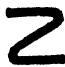
\includegraphics[keepaspectratio]{images/part002_764ec905.jpg}}

把“群”换成“环”、“子群”换成“理想”（左理想或右理想），就得到类似的结果；关于模与代数的类似结果，我们留给读者去陈述。

\subsection{拓扑群与带算子空间的逆极限}

我们将说，逆系统 \((\mathbf{G}_{\alpha}, f_{\alpha\beta})\) 是一个拓扑群的逆系统，如果诸 \(G_{\alpha}\) 是拓扑群且诸 \(f_{\alpha\beta}\) 是连续同态。此时 \(G = \varprojlim G_{\alpha}\) 是积群 \(\prod_{\alpha} G_{\alpha}\) 的一个子群；若给 G 赋以由 \(\prod_{\alpha} G_{\alpha}\) 诱导的拓扑群结构，则如此得到的拓扑群称为拓扑群的逆系统 \((\mathbf{G}_{\alpha}, f_{\alpha\beta})\) 的逆极限。若诸 \(G_{\alpha}\) 是豪斯多夫的（相应地，豪斯多夫且完备的），则 G 是豪斯多夫的且在 \(\prod_{\alpha} G_{\alpha}\) 中闭（相应地，豪斯多夫且完备的）（第一章，§ 8，第 2 节，命题 7 的推论 2 以及第二章，§ 3，第 5 节，命题 10 的推论）。

若 \((\mathbf{G}_{\alpha}^{\prime}, f_{\alpha\beta}^{\prime})\) 是另一个拓扑群的逆系统，且对每个 \(\alpha\) ，\(u_{\alpha}: G_{\alpha} \to G_{\alpha}^{\prime}\) 是一个连续同态，使得诸 \(u_{\alpha}\) 构成映射的逆系统，则 \(u = \varprojlim u_{\alpha}\) 是 G 到 \(G^{\prime} = \varprojlim G_{\alpha}^{\prime}\) 中的一个连续同态（第一章，§ 4，第 4 节）。当把“拓扑群”换成“拓扑环”时，同样的结果成立；关于拓扑模的类似结果，我们留给读者去陈述（§ 6，第 6 节）。

设 \((\mathbf{X}_{\alpha}, g_{\alpha \beta})\) 是拓扑空间的逆系统，\((\mathbf{G}_{\alpha}, f_{\alpha \beta})\) 是拓扑群的逆系统。设每个 \(\mathbf{G}_{\alpha}\) 连续地作用于 \(\mathbf{X}_{\alpha}\) （§ 2，第 4 节），且关系 (1) 对所有 \(x_{\beta} \in \mathbf{X}_{\beta}\) 、\(s_{\beta} \in \mathbf{G}_{\beta}\) 与 \(\alpha \leqslant \beta\) 成立。我们已经看到（第 1 节），\(\mathbf{X} = \varprojlim \mathbf{X}_{\alpha}\) 以 \(\mathbf{G} = \varprojlim \mathbf{G}_{\alpha}\) 为算子群；而且 \(\mathbf{G}\) 连续地作用于 \(\mathbf{X}\) 。因为，若 \(g_{\alpha}\) （相应地，\(f_{\alpha}\) ）是典范映射 \(\mathbf{X} \to \mathbf{X}_{\alpha}\) （相应地，\(\mathbf{G} \to \mathbf{G}_{\alpha}\) ），则按定义

\[
g _ {\alpha} (s, x) = f _ {\alpha} (s). g _ {\alpha} (x)
\]

因而诸映射 \((s.x) \to g_{\alpha}(s.x)\) 在 \(\mathbf{X} \times \mathbf{G}\) 上连续，这表明 \((s, x) \to (s.x)\) 的连续性（第一章，§ 4，第 4 节）。

映射 \(h_{\alpha}: \mathbf{X} / \mathbf{G} \to \mathbf{X}_{\alpha} / \mathbf{G}_{\alpha}\) （它由 \(f_{\alpha}\) 与 \(g_{\alpha}\) 诱导）因此是连续的（§ 2，第 4 节），而映射 \(h: \mathbf{X} / \mathbf{G} \to \varprojlim \mathbf{X}_{\alpha} / \mathbf{G}_{\alpha}\) （它由诸 \(h_{\alpha}\) 定义）也是连续的（第一章，§ 2，第 3 节，命题 4）。

命题 1. 设诸 \(\mathbf{X}_{\alpha}\) 与诸 \(\mathbf{G}_{\alpha}\) 满足上述假设。a) 若 \(\mathbf{X}_{\alpha}\) 的每一点的稳定子群都是 \(\mathbf{G}_{\alpha}\) 的一个紧子群（对每个 \(\alpha \in \mathbf{I}\) ），则每一点 \(x = (x_{\alpha})\) （属于 \(\mathbf{X}\) ）的稳定子群是 \(\mathbf{G}\) 的一个紧子群；\(x\) 的轨道（关于 \(\mathbf{G}\) 的）典范地同胚于诸 \(x_{\alpha}\) 的轨道（关于 \(\mathbf{G}_{\alpha}\) 的）的逆极限；且典范映射 \(h: \mathbf{X} / \mathbf{G} \to \varprojlim \mathbf{X}_{\alpha} / \mathbf{G}_{\alpha}\) 是单射的。

\begin{enumerate}
\def\labelenumi{\alph{enumi})}
\setcounter{enumi}{1}
\tightlist
\item
  若对每个 \(\alpha \in \mathbf{I}\) ，\(\mathbf{X}_{\alpha}\) 的点的每个轨道（关于 \(\mathbf{G}_{\alpha}\) 的）都是紧的，则 \(\mathbf{X}\) 的点的每个轨道（关于 \(\mathbf{G}\) 的）都是相对紧的，且 \(h\) 是满射的。若此外 \(h\) 还是双射的，则 \(\mathbf{X}\) 的点的每个轨道都是紧的。
\end{enumerate}

设 \(x = (x_{\alpha}) \in \mathbf{X}\) ，且对每个 \(\alpha \in \mathbf{I}\) ，设 \(\mathbf{X}_{\alpha}' = \mathbf{G}_{\alpha}.x_{\alpha}\) 为 \(x_{\alpha}\) 的轨道。若 \(\alpha \leqslant \beta\) ，则由 (1) 及关系 \(g_{\alpha\beta}(x_{\beta}) = x_{\alpha}\) 推出 \(g_{\alpha\beta}(\mathbf{X}_{\beta}') \subset \mathbf{X}_{\alpha}',\) 因而 \((\mathbf{X}_{\alpha}')\) 是诸 \(\mathbf{X}_{\alpha}\) 的子集的一个逆系统。对每个 \(\alpha \in \mathbf{I}\) ，设 \(u_{\alpha}: \mathbf{G}_{\alpha} \to \mathbf{X}_{\alpha}'\) 是连续映射 \(s_{\alpha} \to s_{\alpha}.x_{\alpha}\) ；诸 \(u_{\alpha}\) 构成映射的逆系统，而 \(u = \varprojlim u_{\alpha}\) 是连续映射 \(s \to s.x\) ，它把 \(G\) 映入子空间 \(X' = \varprojlim X_{\alpha}'\) （含于 \(X\) ）。a) 的假设蕴含 \(\overline{u}_{\alpha}^{-1}(y_{\alpha})\) 对每个 \(y_{\alpha} \in X_{\alpha}'\) 是紧的。由于 \(u_{\alpha}\) 还是满射的，第一章 § 9 第 6 节命题 8 推论 2 的条件得到满足，因而 a) 的前两个断言成立。于是，若 \(x = (x_{\alpha})\) 与 \(y = (y_{\alpha})\) 使得 \(x_{\alpha}\) 与 \(y_{\alpha}\) 属于关于 \(G_{\alpha}\) 的同一轨道（对每个 \(\alpha \in I\) ），则 \(x\) 与 \(y\) 属于关于 \(G\) 的同一轨道，因此 \(h\) 是单射的。

同样，b) 的假设蕴含：典范映射 \(v_{\alpha}: \mathbf{X}_{\alpha} \to \mathbf{X}_{\alpha}/\mathbf{G}_{\alpha}\) 的逆系统满足第一章 § 9 第 6 节命题 8 推论 2 的条件，因而其逆极限 \(v = \varprojlim v_{\alpha}: \mathbf{X} \to \varprojlim \mathbf{X}_{\alpha}/\mathbf{G}_{\alpha}\) 是满射的，且每一点在 \(v\) 下的逆像都是紧的，这里点取遍 \(\varprojlim X_{\alpha}/G_{\alpha}\) 。由于 \(v\) 分解为

\[
\mathrm{X} \xrightarrow {\psi} \mathrm{X} / \mathrm{G} \xrightarrow {h} \varprojlim \mathrm{X} _ {\alpha} / \mathrm{G} _ {\alpha},
\]

其中 \(\psi\) 是典范映射，b) 的各断言由此得出。

推论 1. 若诸 \(\mathbf{G}_{\alpha}\) 是紧的而诸 \(\mathbf{X}_{\alpha}\) 是豪斯多夫的，则 a) 与 b) 的结论成立。

因为 a) 与 b) 的假设都满足：\(G_{\alpha}\) 的每个闭子群都是紧的，且 \(u_{\alpha}: s_{\alpha} \to s_{\alpha}.x_{\alpha}\) 是紧空间到豪斯多夫空间中的连续映射。

推论 2. 若对每个 \(\alpha \in I\) ，群 \(G_{\alpha}\) 传递地作用于空间 \(X_{\alpha}\) ，且 \(X_{\alpha}\) 的每一点的稳定子群都是 \(G_{\alpha}\) 的紧子群，则 \(G\) 传递地作用于 \(X\)，且 \(X\) 的每一点的稳定子群都是 \(G\) 的紧子群。

因为假设 \(a)\) 满足，且 \(\mathbf{X}_{\alpha}^{\prime} = \mathbf{X}_{\alpha}\) （对每个 \(\alpha\) ）。

推论 3. 设诸 \(\mathbf{G}_{\alpha}\) 是豪斯多夫的。对每个 \(\alpha \in \mathbf{I}\) ，设 \(\mathbf{K}_{\alpha}\) 是 \(\mathbf{G}_{\alpha}\) 的一个紧子群，使得 \(f_{\alpha \beta}(\mathbf{K}_{\beta}) \subset \mathbf{K}_{\alpha}\) 对一切 \(\alpha \leqslant \beta\) 成立。那么，若 \(\mathbf{K} = \varprojlim \mathbf{K}_{\alpha}\) ，则典范映射 \(h\) （它把齐性空间 \(\mathbf{G} / \mathbf{K}\) 映到 \(\varprojlim \mathbf{G}_{\alpha} / \mathbf{K}_{\alpha}\) 中）是一个同胚。

\(h\) 是双射这一事实由推论 1 得出，只需把 \(\mathbf{X}_{\alpha}\) 换成 \(\mathbf{G}_{\alpha}\) ，并把 \(\mathbf{G}_{\alpha}\) 换成以右平移作用的 \(\mathbf{K}_{\alpha}\) （§ 2，第 5 节）。设 \(\varphi\) 是典范映射 \(\mathbf{G} \to \mathbf{G} / \mathbf{K}\) ，且对每个 \(\alpha\) ，设 \(f_{\alpha}\) 是典范映射 \(\mathbf{G} \to \mathbf{G}_{\alpha}\) 。若对每个 \(\alpha, \mathbf{V}_{\alpha}\) 取遍 \(e_{\alpha}\) （\(\mathbf{G}_{\alpha}\) 的单位元）的邻域组成的一个基本系，则诸集合 \(\mathbf{V} = \overline{f}_{\alpha}^{-1}(\mathbf{V}_{\alpha}) (\alpha \text{与} \mathbf{V}_{\alpha} \text{变动})\) 构成 \(e\) （\(\mathbf{G}\) 的单位元）的邻域基本系（第一章，§ 4，第 4 节，命题 9），而诸集合 \(\varphi(\mathbf{V}.K)\) 构成 \(\varphi(e)\) 在 \(G/K\) 中的邻域基本系。我们要证明 \(\varphi(V.K)\) 在 \(h\) 下的像包含 \(h(\varphi(e))\) 的一个邻域，亦即存在 \(\beta \geqslant \alpha\) 和一个邻域 \(W_{\beta}\) （\(e_{\beta}\) 在 \(G_{\beta}\) 中），使得 \(\overline{f}_{\beta}^{-1}(W_{\beta}.K_{\beta}) \subset V.K\) 。现在，关系 \(x \in V.K\) 等价于存在 \(y\) （属于 \(K\) ），使 \(f_{\alpha}(xy^{-1}) \in V_{\alpha}\) ，即 \(f_{\alpha}(x) \in V_{\alpha}.f_{\alpha}(K)\) ；从而 \(V.K = \overline{f}_{\alpha}^{-1}(V_{\alpha}.f_{\alpha}(K))\) 。令 \(U_{\alpha} = V_{\alpha}.f_{\alpha}(K)\) ；我们将看到，存在 \(\beta \geqslant \alpha\) ，使得当令 \(U_{\beta} = \overline{f}_{\alpha\beta}^{-1}(U_{\alpha})\) 时有 \(K_{\beta} \subset U_{\beta}\) ；于是将可推出存在一个邻域 \(W_{\beta}\) （\(e_{\beta}\) 在 \(G_{\beta}\) 中），使 \(W_{\beta}.K_{\beta} \subset U_{\beta}\) （第二章，§ 4，第 3 节，命题 4 的推论），而这便建立了所要的关系

\[
\overline {{f}} _ {\beta} ^ {-1} (\mathrm{W} _ {\beta}. \mathrm{K} _ {\beta}) \subset \overline {{f}} _ {\beta} ^ {-1} (\mathrm{U} _ {\beta}) = \mathrm{V}. \mathrm{K}.
\]

我们用反证法来进行：对每个 \(\beta \geqslant \alpha\) ，用 \(\mathbf{M}_{\beta}\) 表示 \(\mathbf{K}_{\beta} \cap \mathbb{C}\mathbf{U}_{\beta}\) ；由于 \(\overline{f}_{\beta \gamma}^{-1}(\mathrm{U}_{\beta}) = \mathrm{U}_{\gamma}\) （当 \(\alpha \leqslant \beta \leqslant \gamma\) 时），诸 \(\mathbf{M}_{\beta}\) 构成诸 \(\mathbf{G}_{\beta}\) 的紧子集的一个逆系统（对 \(\beta \geqslant \alpha\) ）。如果它们都非空，则它们的逆极限 \(\mathbf{M}\) 也非空（第一章，§ 9，第 6 节，命题 8）。显然 \(\mathbf{M} \subset \mathbf{K}\) 且 \(f_{\alpha}(\mathbf{M}) \subset \mathbf{M}_{\alpha}\) ；但这是荒谬的，因为 \(f_{\alpha}(\mathbf{K}) \subset \mathbf{U}_{\alpha}\) ，于是证明完毕。

\subsection{拓扑群的逼近}

设 G 是一个群，并设 \((\mathrm{H}_{\alpha})_{\alpha\in\mathbf{I}}\) 是 G 的正规子群的一个族，使得 \(H_{\alpha}\supset H_{\beta}\) 对一切 \(\alpha\leqslant\beta\) 成立。对每个 \(\alpha\in I\) ，令 \(G_{\alpha}=G/H_{\alpha}\) ；而对 \(\alpha\leqslant\beta\) ，令 \(f_{\alpha\beta}\) 为典范同态 \(G/H_{\beta}\to G/H_{\alpha}\) ，它因而把 \(H_{\beta}\) 在 G 中的一个陪集 T 映为陪集 \(TH_{\alpha}\) （\(H_{\alpha}\) 在 G 中的）。显然 \((G_{\alpha},f_{\alpha\beta})\) 是群的一个逆系统；\(\tilde{G}=\varprojlim G_{\alpha}\) 的元素是诸族 \((T_{\alpha})_{\alpha\in\mathbf{I}}\) ，其中 \(T_{\alpha}\) 是 \(H_{\alpha}\) 在 G 中的一个陪集（对每个 \(\alpha\) ），且 \(T_{\alpha}\supset T_{\beta}\) 对一切 \(\alpha\leqslant\beta\) 成立。映射 \(i:s\to(sH_{\alpha})\) （它把 G 映入 \(\tilde{G}\) ）是诸典范同态 \(G\to G/H_{\alpha}\) 的逆极限，因而是 G 到 \(\tilde{G}\) 中的一个同态，且元素 \((T_{\alpha})\in\tilde{G}\) 在 i 下的逆像等于 \(\bigcap_{\alpha\in I}T_{\alpha}\) 。于是 i 的核是 \(\bigcap_{\alpha\in I}H_{\alpha}\) ，而 i 的像由交非空的诸族 \((T_{\alpha})\in\tilde{G}\) 组成。

现在设 G 是一个拓扑群；若给每个 \(G_{\alpha} = G/H_{\alpha}\) 赋以商拓扑，则显然 \((\mathbf{G}_{\alpha}, f_{\alpha\beta})\) 是拓扑群的一个逆系统，且 \(i : G \to \tilde{G}\) 是一个连续同态。

命题 2. 设 G 是一个拓扑群，并设 \((\mathrm{H}_{\alpha})_{\alpha\in I}\) 是 G 的正规子群的一个族，使得 \(H_{\alpha}\supset H_{\beta}\) 对一切 \(\alpha\leqslant\beta\) 成立，且满足下面的条件：

(AP) 对每个 \(\alpha \in I\) ，\(H_{\alpha}\) 在 G 中闭，且 G 中单位元 \(e\) 的每个邻域都包含诸 \(H_{\alpha}\) 之一（换言之，诸 \(H_{\alpha}\) 组成的滤基收敛于 \(e\) ）。

那么，映射 \(i: \mathbf{G} \to \tilde{\mathbf{G}} = \varprojlim \mathbf{G} / \mathbf{H}_{\alpha}\) 是 \(\mathbf{G}\) 到 \(i(\mathbf{G})\) 上的一个严格态射；\(\tilde{\mathbf{G}}\) 是豪斯多夫的，且 \(i(\mathbf{G})\) 在 \(\tilde{\mathbf{G}}\) 中稠密；最后，\(i\) 的核是 \(\{e\}\) 在 \(\mathbf{G}\) 中的闭包。此外，若诸 \(\mathbf{H}_{\alpha}\) 中有一个是完备的，则 \(i\) 是满射的。

显然诸 \(G_{\alpha} = G/H_{\alpha}\) 是豪斯多夫的（§ 2，第 5 节，命题 13），因而 \(\tilde{G}\) 也是（因为它是 \(\prod_{\alpha \in I} G_{\alpha}\) 的一个子空间）。i 的核 H 是诸 \(H_{\alpha}\) 的交，因而是 G 的一个闭子群。由于 \(e\) 的每个邻域都包含某个 \(H_{\alpha}\) ，它包含 \(H\) ，因此{[}§ 3，第 1 节，公式 (1){]}\(H\) 是 \(\{e\}\) 的闭包。接下来我们证明 \(i(G)\) 在 \(\tilde{G}\) 中稠密。设 \(f_{\alpha}\) 是典范映射 \(\tilde{G} \to G_{\alpha}\) ，它是 \(\tilde{G}\) 上射影 \(pr_{\alpha}\) 的限制；\(\varphi_{\alpha} = f_{\alpha} \circ i\) 是典范映射 \(G \to G / H_{\alpha}\) 。若 \(U\) 是 \(\tilde{G}\) 的任一非空开集，则存在指标 \(\alpha \in I\) 与非空开集 \(U_{\alpha}\) （在 \(G_{\alpha}\) 中），使得 \(\overline{f}_{\alpha}^{-1}(U_{\alpha}) \subset U\) （第一章，§ 4，第 4 节，命题 9）；因而

\[
\overline {{i}} ^ {-1} (\mathbf {U}) \supset \overline {{\varphi}} _ {\alpha} ^ {-1} (\mathbf {U} _ {\alpha});
\]

但由于 \(\varphi_{\alpha}\) 是满射的，\(\overline{i}^{-1}(\mathbf{U})\) 非空，因而 \(i(\mathbf{G}) \cap \mathbf{U} \neq \emptyset\) 。为看出 \(i\) 是 \(\mathbf{G}\) 到 \(i(\mathbf{G})\) 上的一个严格态射，考虑一个邻域 \(\mathbf{V}\) （\(e\) 在 \(\mathbf{G}\) 中的）。存在一个邻域 \(\mathbf{W}\) （\(e\) 在 \(\mathbf{G}\) 中的），使得 \(\mathbf{W}^2 \subset \mathbf{V}\) ，又存在指标 \(\alpha \in \mathbf{I}\) ，使得 \(\mathbf{H}_{\alpha} \subset \mathbf{W}\) ；由此推出 \(\mathbf{V}\) 包含 \(\mathrm{WH}_{\alpha} = \overline{\varphi}_{\alpha}^{-1}(\varphi_{\alpha}(\mathbf{W})) = \overline{i}^{-1}(\overline{f}_{\alpha}^{-1}(\varphi_{\alpha}(\mathbf{W})))\) 。由于 \(\overline{f}_{\alpha}^{-1}(\varphi_{\alpha}(\mathbf{W}))\) 是 \(\tilde{\mathbf{G}}\) 中单位元的一个邻域，结论得证。

最后，假设存在指标 \(\gamma \in I\) ，使得 \(H_{\gamma}\) 是完备的。为证明 \(i\) 是满射的，只需证明每个族 \((T_{\alpha})_{\alpha \in I} \in \tilde{G}\) 有非空的交。由于 \(T_{\gamma}\) 是由 \(H_{\gamma}\) 经平移得到的，它是 \(G\) 的一个完备子空间（关于右一致结构与左一致结构两者）。此外，由于每个邻域 \(U\) （\(e\) 在 \(G\) 中的）都包含诸 \(H_{\alpha}\) 之一，相应的集合 \(T_{\alpha}\) 是 \(U_{d-}\) （或 \(U_{s-}\) ）小的，因而诸 \(T_{\alpha}\) （含于 \(T_{\gamma}\) 者）所成之集是一个柯西滤基；故它在 \(T_{\gamma}\) 中收敛，又由于诸 \(T_{\alpha}\) 在 \(G\) 中闭（因为它们是诸 \(H_{\alpha}\) 的平移），它们的交非空。

证毕。

推论 1. 若条件 (AP) 满足，且此外诸（豪斯多夫）群 \(\mathbf{G} / \mathbf{H}_{\alpha}\) 都是完备的，则群 \(\mathbf{G}\) 有一个可等同于 \(\tilde{\mathbf{G}}\) 的豪斯多夫完备化；且映射 \(i: \mathbf{G} \to \tilde{\mathbf{G}}\) 那时可等同于典范映射（§ 3，第 3 节，命题 5）。

因为此时 \(\tilde{\mathbf{G}}\) 是完备的（第 2 节），且命题 2 表明 \(i(\mathbf{G})\) 同构于由 \(\mathbf{G}\) 得到的豪斯多夫群；由于它在 \(\tilde{\mathbf{G}}\) 中稠密，推论得证（\(\S 3\) ，第 3 节，命题 5）。特别地：

推论 2. 设 G 是一个群，并设 \((\mathrm{H}_{\alpha})\) 是 G 的正规子群的一个族，它关于关系 \(\mathrm{H}_{\alpha} \supset \mathrm{H}_{\beta}\) 有向。若给 G 赋以使诸 \(\mathrm{H}_{\alpha}\) 构成单位元 \(e\) 的邻域基本系的群拓扑，则 G 的相伴豪斯多夫群同构于 \(\mathrm{G}_{1} = \mathrm{G} / \left( \bigcap_{\alpha} \mathrm{H}_{\alpha} \right)\) ；\(\mathrm{G}_{1}\) 有一个完备化 \(\hat{\mathrm{G}}_{1} = \tilde{\mathrm{G}}\) ；且典范映射 \(\mathrm{G}_{1} \to \hat{\mathrm{G}} = \varprojlim \mathrm{G} / \mathrm{H}_{\alpha}\) 可延拓为 \(\hat{\mathrm{G}} = \hat{\mathrm{G}}_{1}\) 到 \(\tilde{\mathrm{G}}\) 上的一个同构。

G 的子群 \(H_{\alpha}\) 是开的，因而也是闭的（\(\S\) 2，第 1 节，命题 4 的推论），且 \(G/H_{\alpha}\) 是离散的（\(\S\) 2，第 6 节，命题 18）；于是推论 1 的条件得到满足。

在本小节的其余部分，我们将假设 G 是豪斯多夫的，且 \((\mathbf{H}_{\alpha})\) 是 G 的紧正规子群的一个族，它关于关系 \(H_{\alpha} \supset H_{\beta}\) 有向并满足条件 (AP)；根据命题 2，映射

\[
i: \mathrm{G} \rightarrow \tilde {\mathrm{G}} = \varprojlim \mathrm{G} / \mathrm{H} _ {\alpha}
\]

于是是一个拓扑群的同构，它使我们可以把 G 与 \(\tilde{G}\) 等同起来。我们用 \(f_{\alpha}\) 表示典范映射 \(G \rightarrow G/H_{\alpha}\) 。

引理 1. 在命题 2 的假设下，若 E 是 G 的任一闭子集，我们有 \(\mathbf{E} = \bigcap_{\alpha} \mathrm{EH}_{\alpha}\) 。

因为 E 是诸集合 EV 的交，这里 V 取遍 e 的邻域滤子{[}§ 3，第 1 节，公式 (1){]}，且 e 的每个邻域都包含某个 \(H_{\alpha}\) ；又因 \(E \subset EH_{\alpha}\) ，结论得证。

命题 3. 假设 G 是豪斯多夫的，且诸 \(H_{\alpha}\) 是紧的并满足 (AP)。

\begin{enumerate}
\def\labelenumi{\alph{enumi})}
\item
  设 L 是 G 的一个闭子群；则对每个 \(\alpha\in I\) ，子群 \(L_{\alpha}=f_{\alpha}(L)\) （\(G_{\alpha}=G/H_{\alpha}\) 中的）是闭的，且 G 到 \(\varprojlim G_{\alpha}\) 上的同构 i 经限制给出 L 到 \(\varprojlim L_{\alpha}\) 上的一个同构。若还有 L 在 G 中正规，则 \(L_{\alpha}\) 在 \(G_{\alpha}\) 中正规（对每个 \(\alpha\in I\) ），且过渡到商，i 诱导出 G/L 到 \(\varprojlim G_{\alpha}/L_{\alpha}\) 上的一个同构。
\item
  反之，对每个 \(\alpha \in I\) ，设 \(L_{\alpha}\) 是 \(G_{\alpha}\) 的一个闭子群，使得 \(L_{\alpha} = f_{\alpha \beta}(L_{\beta})\) 对一切 \(\alpha \leqslant \beta\) 成立。则存在唯一的闭子群 \(L\) （\(G\) 中的），使得 \(L_{\alpha} = f_{\alpha}(L)\) 对每个 \(\alpha \in I\) 成立；而若此外 \(L_{\alpha}\) 在 \(G_{\alpha}\) 中正规（对每个 \(\alpha \in I\) ），则 \(L\) 在 \(G\) 中正规。
\item
  由于 \(\mathbf{H}_{\alpha}\) 是紧的，\(\mathrm{LH}_{\alpha}\) 在 \(\mathbf{G}\) 中闭（\(\S 4\) ，第 1 节，命题 1 的推论 1），因而 \(\mathbf{L}_{\alpha}\) 在 \(\mathbf{G}_{\alpha}\) 中闭。由于 \(i\) 把拓扑群 \(\mathbf{G}\) 与 \(\varprojlim \mathbf{G}_{\alpha}\) 等同起来，且 \(\varprojlim \mathbf{L}_{\alpha}\) 可与 \(\varprojlim \mathbf{G}_{\alpha}\) 的一个（拓扑）子群等同，\(i\) 把子群 \(\bigcap_{\alpha} \mathrm{LH}_{\alpha}\) （\(\mathbf{G}\) 的）与 \(\varprojlim \mathbf{L}_{\alpha}\) 等同起来，而为证明第一个断言，只需注意由引理 1 有 \(\mathbf{L} = \bigcap_{\alpha} \mathrm{LH}_{\alpha}\) 。另一方面，若 \(\mathbf{L}\) 正规，则对每个 \(\alpha \in \mathbf{I}\) ，映射 \(f_{\alpha}': \mathbf{G} / \mathbf{L} \to \mathbf{G}_{\alpha} / \mathbf{L}_{\alpha}\) （它由 \(f_{\alpha}\) 诱导）是一个满射的严格态射（\(\S 2\) ，第 8 节，注 3），其核是紧正规子群 \(\mathrm{H}_{\alpha} \mathrm{L} / \mathrm{L}\) （\(\mathrm{G} / \mathrm{L}\) 的），即紧子群 \(\mathrm{H}_{\alpha}\) （\(\mathbf{G}\) 的）的典范像。由于诸子群 \(\mathrm{H}_{\alpha} \mathrm{L} / \mathrm{L}\) （\(\mathrm{G} / \mathrm{L}\) 的）满足条件 (AP)（§ 2，第 8 节，命题 24），且 G/L 是豪斯多夫的，a) 的最后一个断言是命题 2 的推论。
\item
  设 \(f_{\alpha \beta}'\) 是 \(f_{\alpha \beta}\) 到 \(\mathbf{L}_{\beta} (\alpha \leqslant \beta)\) 上的限制。则 \((\mathbf{L}_{\alpha}, f_{\alpha \beta}')\) 是拓扑群的一个逆系统，其逆极限 \(\mathbf{L}\) 可与子群 \(\mathbf{G} \cap \prod_{\alpha} \mathbf{L}_{\alpha}\) （\(\mathbf{G}\) 的）等同。据假设，\(f_{\alpha \beta}'\) 是满射的，且其核是紧子群 \(f_{\beta}(\mathrm{H}_{\alpha}) \cap \mathrm{L}_{\beta}\) （\(\mathbf{L}_{\beta}\) 的）；因而（第一章，§ 9，第 6 节，命题 8 的推论 1）我们有 \(\mathbf{L}_{\alpha} = f_{\alpha}(\mathbf{L})\) ，对一切 \(\alpha \in \mathbf{I}\) 成立。若 \(\mathbf{L}'\) 是 \(\mathbf{G}\) 的另一个闭子群，使得 \(f_{\alpha}(\mathbf{L}') = \mathbf{L}_{\alpha}\) 对一切 \(\alpha \in \mathbf{I}\) 成立，则 \(\mathbf{L}'\mathbf{H}_{\alpha} = \overline{f}_{\alpha}^{-1}(\mathbf{L}_{\alpha})\) ，从而（引理 1）\(\mathbf{L}' = \bigcap_{\alpha} \mathbf{L}'\mathbf{H}_{\alpha} = \bigcap_{\alpha} \overline{f}_{\alpha}^{-1}(\mathbf{L}_{\alpha}) = \mathbf{L}\) 。最后，b) 的最后一个断言由公式 \(\mathbf{L} = \bigcap_{\alpha} \overline{f}_{\alpha}^{-1}(\mathbf{L}_{\alpha})\) 得出，因为诸 \(\overline{f}_{\alpha}^{-1}(\mathbf{L}_{\alpha})\) 现在是 \(\mathbf{G}\) 的正规子群。
\end{enumerate}

命题 4. 假设 G 是豪斯多夫的，诸 \(H_{\alpha}\) 是紧的，且 (AP) 满足。若 \(C_{\alpha}\) 是 \(G_{\alpha} = G/H_{\alpha}\) 的单位分量，则 G 的单位分量 C 可与 \(\varprojlim C_{\alpha}\) 等同，且我们有 \(f_{\alpha}(C) = C_{\alpha}\) 。本命题是下述引理的推论：

引理 2. 设 G 是一个豪斯多夫拓扑群，H 是 G 的一个紧正规子群，\(\varphi\) 是典范映射 \(\mathbf{G} \to \mathbf{G} / \mathbf{H}\) 。若 C 是 G 的单位分量，则 \(\varphi(\mathbf{C})\) 是 \(\mathbf{G}' = \mathbf{G} / \mathbf{H}\) 的单位分量。

一旦建立了这个引理，我们就将有 \(f_{\alpha}(\mathbf{C}) = \mathbf{C}_{\alpha}\) （对每个 \(\alpha \in \mathbf{I}\) ），且由于 \(\mathbf{C}\) 是 \(\mathbf{G}\) 的一个闭子群（§ 2，第 2 节，命题 7），只需应用命题 3a)。

为证明引理，首先注意，若 \(C'\) 是 \(e'\) 在 \(G'\) 中的连通分量，则 \(\varphi(C) \subset C'\) ，因为 \(\varphi(C)\) 是连通的。假设 \(\varphi(C) \neq C'\) 。由于 C 是 G 的一个闭正规子群（§2，第 2 节，命题 7），\(\varphi(C)\) 是 \(G'\) 的一个正规子群；若 \(\psi\) 是典范映射 \(G' \to G'/\varphi(C)\) ，则 \(\psi(C')\) 是连通的且不只由单位元组成；因而 \(G'/\varphi(C)\) 的单位分量不只由单位元组成。但 \(G'/\varphi(C)\) 同构于 \((G/H)/(HC/H)\) ，从而同构于 G/HC，于是也同构于 \((G/C)/(HC/C)\) （§2，第 7 节，命题 22 的推论以及命题 20）。现在，G/C 是豪斯多夫的且全不连通的（第一章，§11，第 5 节，命题 9），而 HC/C 作为 G 的紧正规子群 H 的典范像，是 G/C 的一个紧子群。因此只需在附加假设 G 全不连通、即 \(C = \{e\}\) 之下证明引理 2。

于是设 \(C' \neq \{e'\}\) ；把 G 换成它的子群 \(\varphi^{-1}(C')\) （它全不连通且包含 H），我们就可以假设 \(G'\) 是连通的且不止由一点组成。

设 \(\mathfrak{M}\) 是由闭子群 \(L\) （\(G\) 中的）组成的集合，这些子群满足 \(LH = G\) 。我们将证明 \(\mathfrak{M}\) 按关系 \(\supset\) 排序是归纳的。事实上，若 \(\mathfrak{X}\) 是 \(\mathfrak{M}\) 的一个线性有序子集，则对每个 \(x \in G\) ，诸集合 \(xH \cap L\) （\(L \in \mathfrak{X}\)）组成的集是一个由紧空间 \(xH\) 中的闭集组成的滤基；因而这些集合的交非空，这表明诸子群 \(L \in \mathfrak{X}\) 的交属于 \(\mathfrak{M}\) 。应用佐恩引理，我们因此看出 \(\mathfrak{M}\) 有一个极小元 \(L_0\) 。由于 \(H\) 是紧的，\(G/H = L_0H/H\) 同构于 \(L_0/(L_0 \cap H)\) （\(\S 4\) ，第 1 节，命题 1 的推论 3）；由于 \(L_0\) 全不连通且 \(L_0 \cap H\) 是紧的，我们看出可以把 \(G\) 换成 \(L_0\) ；换言之，我们可以附加假设不存在闭子群 \(L \neq G\) 满足 \(LH = G\) 。

现在设 F 是 G 中既开又闭的单位元的诸邻域的交，我们来证明 F 是 G 的一个闭子群。显然 F 在 G 中闭；因而只需证明 \(F^{-1}.F \subset F\) 。但若 \(x \in F\) 且 V 是 e 在 G 中的一个既开又闭的邻域，则 xV 也是；否则 e 将属于 xV 在 G 中的余集 W，而 W 又是既开又闭的，且我们将有 \(x \notin W\) ；从而 \(x \notin F\) ，与假设矛盾。由此推出 xF（诸集合 xV 的交，V 取遍 e 在 G 中的既开又闭的邻域）包含 F；换言之，\(x^{-1}F \subset F\) ，这就证明了我们的断言。由于 G 全不连通且 \(G \neq \{e\}\) ，我们有 \(F \neq G\) 。但若 V 是 e 在 G 中的一个既开又闭的邻域，则 VH 在 G 中也是既开又闭的（§ 4，第 1 节，命题 1 的推论 1），因而 \(\varphi(V)\) 在 G/H 中既开又闭，而这在假设之下蕴含 \(\varphi(V) = G/H\) 。我们将由此推出 FH = G，它将给出所要的矛盾并完成引理的证明。事实上，对每个 \(x \in G\) ，xH 与 e 的每个既开又闭的邻域 V 相交，因而也与这些邻域的交 F 相交，因为诸集合 \(Vx \cap H\) 组成一个由紧空间 xH 中的闭集组成的滤基。

证毕。

注. 若子群 \(H_{\alpha}\) 对某个 \(\alpha \in I\) 是紧的，则 \(H_{\beta}\) 对一切 \(\beta \geqslant \alpha\) 是紧的，因为它是 \(H_{\alpha}\) 的一个闭子群。由于所有 \(\beta \in I\) （满足 \(\beta \geqslant \alpha\) 的）组成的集合在 I 中共尾，在群 G 的研究中，假设诸 \(H_{\alpha}\) 之一是紧的与假设所有 \(H_{\alpha}\) 都是紧的，本质上有同样的结果。

\subsection{在逆极限上的应用}

命题 5. 设 \((\mathbf{G}_{\alpha}, f_{\alpha \beta})\) 是豪斯多夫拓扑群的一个逆系统，使得诸 \(f_{\alpha \beta}\) 是核紧的满射严格态射。则对每个 \(\alpha \in I\) ，典范映射 \(f_{\alpha}\) （它把 \(\mathbf{G} = \varprojlim \mathbf{G}_{\alpha}\) 映入 \(\mathbf{G}_{\alpha}\) ）是一个核紧的满射严格态射。

\(f_{\alpha}\) 是满射的且其核是紧的这两件事是第一章 § 9 第 6 节命题 8 推论 1 的推论。剩下的只是证明 \(f_{\alpha}\) 是一个严格态射。用 \(e\) （相应地，\(e_{\alpha}\) ）表示 G （相应地，\(G_{\alpha}\) ）的单位元。G 中 \(e\) 的每个邻域 V 包含形如 \(\overline{f}_{\beta}^{-1}(V_{\beta})\) 的集合，这里 \(V_{\beta}\) 是 \(e_{\beta}\) 在 \(G_{\beta}\) 中的一个邻域，且我们可以假设 \(\beta \geqslant \alpha\) ；由于 \(f_{\alpha \beta}\) 是满射的严格态射，\(f_{\alpha \beta}(V_{\beta})\) 是 \(e_{\alpha}\) 在 \(G_{\alpha}\) 中的一个邻域，又由于 \(f_{\beta}\) 是满射的，我们有 \(V_{\beta} \subset f_{\beta}(V)\) ，由此

\[
f _ {\alpha} (\mathbf {V}) = f _ {\alpha \beta} (f _ {\beta} (\mathbf {V})) \supset f _ {\alpha \beta} (\mathbf {V} _ {\beta});
\]

这表明 \(f_{\alpha}(\mathbf{V})\) 是 \(e_{\alpha}\) 在 \(\mathbf{G}_{\alpha}\) 中的一个邻域。

若 \(\mathrm{H}_{\alpha}=\overline{f}_{\alpha}^{-1}(e_{\alpha})\) ，则每个 \(H_{\alpha}\) 是 G 的一个紧正规子群；诸 \(H_{\alpha}\) 显然满足第 3 节的条件 (AP)；且 \(G_{\alpha}\) 可与 \(G/H_{\alpha}\) 等同。特别地，第 3 节的命题 3 与命题 4 可应用于 G 与诸 \(H_{\alpha}\) 。

推论 1. 设 \((\mathbf{G}_{\alpha}, f_{\alpha \beta})\) 是满足命题 5 的假设的拓扑群逆系统；设 \((\mathbf{G}_{\alpha}', f_{\alpha \beta}')\) 是拓扑群的一个逆系统，且对每个 \(\alpha\) ，设 \(u_{\alpha}: \mathbf{G}_{\alpha} \to \mathbf{G}_{\alpha}'\) 是核紧的满射严格态射，使得诸 \(u_{\alpha}\) 构成映射的一个逆系统。则 \(u = \varprojlim u_{\alpha}\) 是 \(\mathbf{G} = \varprojlim \mathbf{G}_{\alpha}\) 到 \(\mathbf{G}' = \varprojlim \mathbf{G}_{\alpha}'\) 上的一个严格态射，且其核是紧的。

设 \(N_{\alpha}\) 是 \(u_{\alpha}\) 的核。\(L_{\alpha} = \overline{f}_{\alpha}^{-1}(N_{\alpha})\) 因而是满射严格态射 \(v_{\alpha} = u_{\alpha} \circ f_{\alpha}: G \to G'_{\alpha}\) 的核；由于 \(L_{\alpha}/H_{\alpha}\) 同构于 \(N_{\alpha}\) （§ 2，第 7 节，命题 20），\(L_{\alpha}\) 是 G 的一个紧正规子群（§ 4，第 1 节，命题 2 的推论 2）。u 的核 L 是诸 \(L_{\alpha}\) 的交。用 \(\varphi\) 表示典范映射 \(G \to G/L\) ；则我们可以写 \(v_{\alpha} = w_{\alpha} \circ \varphi\) ，其中 \(w_{\alpha}\) 是 G/L 到 \(G'_{\alpha}\) 上的一个严格态射，其核是 \(L_{\alpha}/L\) 。由于诸 \(L_{\alpha}/L\) 的交是 G/L 的单位元，且诸 \(L_{\alpha}/L\) 组成一个滤基并且是紧的，这个滤基收敛于 G/L 的单位元（第一章，§ 9，第 1 节，定理 1 的推论）。于是第 3 节的命题 2 表明 \(w = \varprojlim w_{\alpha}\) 是 G/L 到 \(G'\) 上的一个同构；由此推出 \(w \circ \varphi\) 是 G 到 \(G'\) 上的一个严格态射，其核为 L。但显然 \(u = w \circ \varphi\) ，这样推论就证明了。

推论 2. 设 \((\mathbf{G}_{\alpha}, f_{\alpha \beta})\) 是满足命题 5 的条件的拓扑群逆系统，并设 \(\mathbf{G}'\) 是一个拓扑群，其中存在一个邻域 \(\mathbf{V}'\) （单位元 \(e'\) 的），它不含 \(\mathbf{G}'\) 的除 \(\{e'\}\) 外的任何子群。那么，若 \(v: \mathbf{G} \to \mathbf{G}'\) 是任一连续同态，则存在指标 \(\alpha \in \mathbf{I}\) 与连续同态 \(v_{\alpha}: \mathbf{G}_{\alpha} \to \mathbf{G}'\) ，使得 \(v = v_{\alpha} \circ f_{\alpha}\) 。

因为由于 \(\overline{v}^{-1}(\mathbf{V}^{\prime})\) 是 \(e\) 在 \(\mathbf{G}\) 中的一个邻域，存在指标 \(\alpha\) 与一个邻域 \(\mathbf{V}_{\alpha}\) （\(e_{\alpha}\) 在 \(\mathbf{G}_{\alpha}\) 中的），使得 \(\overline{f}_{\alpha}^{-1}(\mathbf{V}_{\alpha}) \subset \overline{v}^{-1}(\mathbf{V}^{\prime})\) 。因而 \(v(\mathbf{H}_{\alpha}) \subset \mathbf{V}^{\prime}\) ，且由于 \(v(\mathbf{H}_{\alpha})\) 是 \(\mathbf{G}^{\prime}\) 的一个子群，由此推出 \(v(\mathbf{H}_{\alpha}) = \{e^{\prime}\}\) 。由于 \(f_{\alpha}\) 可与典范映射 \(\mathbf{G} \to \mathbf{G}/\mathbf{H}_{\alpha}\) 等同，本推论是连续同态的典范分解（§ 2，第 8 节）的推论。

\BourbakiExercises
\BourbakiExerciseGroup

\begin{enumerate}
\def\labelenumi{\arabic{enumi})}
\item
  有限群 G 的与群结构相容的每个拓扑，可以这样得到：取包含 G 的一个正规子群 H 的那些集合作为单位元的邻域。
\item
半拓扑群是指一个群 \(\mathbf{G}\) ，带有一个拓扑，使得对每个 \(a \in \mathbf{G}\) ，平移 \(x \to ax\) 与 \(x \to xa\) 都在 \(\mathbf{G}\) 上连续，且对称 \(x \to x^{-1}\) 在 \(\mathbf{G}(*)\) 上连续。
\end{enumerate}

\begin{enumerate}
\def\labelenumi{\alph{enumi})}
\tightlist
\item
  一个滤子 \(\mathfrak{B}\) （在群 \(\mathbf{G}\) 上）是 \(e\) 的邻域滤子（在使 \(\mathbf{G}\) 成为半拓扑群的一个拓扑中），当且仅当 \(\mathfrak{B}\) 满足公理 \((\mathrm{GV}_{\mathrm{I}})\) 与 \((\mathrm{GV}_{\mathrm{III}})\) ，且滤子族
\end{enumerate}

\[
\mathfrak {B} (x) = x. \mathfrak {B} = \mathfrak {B}. x \quad (x \in G)
\]

满足第一章 § 1 第 2 节的公理 \((\mathbf{V}_{\mathbf{IV}})\) 。

\begin{enumerate}
\def\labelenumi{\alph{enumi})}
\setcounter{enumi}{1}
\tightlist
\item
  若 G 是无限群，试证：以 \(\varnothing\) 与 G 的有限子集的余集为开集的那个拓扑，使 G 成为一个非豪斯多夫的半拓扑群，其中 \(\{e\}\) 是闭的，但与 G 的群结构不相容。
\end{enumerate}

\(^{*}c)\) 在 R 上定义一个比通常拓扑更细的拓扑，使 R 成为一个半拓扑群但不是拓扑群{[}考虑一个递减数列 \((r_{n})\) （诸数 \textgreater0 ，趋于 0），并取诸对称区间 {]}-a, a{[} 与点集 \(\pm r_{n}\) 的余集的交）。 *

(*) 若 G 是局部紧的，这些条件蕴含 G 的拓扑与其群结构相容（第十章，§ 3，习题 25）。

\begin{enumerate}
\def\labelenumi{\arabic{enumi})}
\setcounter{enumi}{2}
\item
  设 A 是半拓扑（相应地，拓扑）群 G 的一个子集。若 V 取遍 G 中 e 的邻域滤子，则诸集合 AV 的交、或诸集合 VA （或诸集合 VAV）的交是 A 的闭包 \(\overline{A}\) 。
\item
  仿拓扑群是指一个群 G ，带有一个满足公理 \((\mathrm{GT}_{\mathbf{I}})(*)\) 的拓扑。
\end{enumerate}

\begin{enumerate}
\def\labelenumi{\alph{enumi})}
\item
  一个滤子 \(\mathfrak{B}\) （群 \(G\) 上的）是 \(e\) 的邻域滤子（对应于使 \(G\) 成为仿拓扑群的一个拓扑），当且仅当 \(\mathfrak{B}\) 满足公理 \((\mathrm{GV}_{\mathbf{I}})\) 与 \((\mathrm{GV}_{\mathbf{III}})\) ，且 \(e \in V\) 对一切 \(V \in \mathfrak{B}\) 成立。相应的拓扑则是唯一的；它是豪斯多夫的，当且仅当诸集合 \(V.V^{-1}\) （\(V\) 取遍 \(\mathfrak{B}\) ）的交仅由点 \(e\) 组成。
\item
  在整数群 \(\mathbf{Z}\) 上，设 \(\mathbf{V}_n\) 是由 \(0\) 与所有整数 \(m \geqslant n\) 组成的集合（对每个 \(n > 0\) ）。试证诸 \(\mathbf{V}_n\) 构成 \(0\) 的邻域基本系（对应 \(\mathbf{Z}\) 上一个非豪斯多夫拓扑），且带此拓扑的 \(\mathbf{Z}\) 是一个仿拓扑群，其中 \(\{0\}\) 是闭的。
\item
  仿拓扑群 G 是拓扑群，当且仅当对 G 的每个子集 A ，诸集合 AV （或诸集合 VA）的交是 A 的闭包 \(\overline{A}\) （当 V 取遍 e 的邻域滤子时）。（为看出条件是充分的，取 A 为 e 的一个开邻域的余集。）
\end{enumerate}

\begin{enumerate}
\def\labelenumi{\arabic{enumi})}
\setcounter{enumi}{4}
\tightlist
\item
  设 \(\mathfrak{B}\) 是群 \(\mathbf{G}\) 上的一个滤子，满足公理 \((\mathrm{GV}_{\mathbf{I}})\) 与 \((\mathrm{GV}_{\mathbf{II}})\) 。
\end{enumerate}

\begin{enumerate}
\def\labelenumi{\alph{enumi})}
\tightlist
\item
  存在唯一的拓扑 \(\mathfrak{C}_s\) （相应地，\(\mathfrak{C}_d\) ），它定义在 \(\mathbf{G}\) 上，使得对每个 \(a \in \mathbf{G}\) ，\(a\) 关于 \(\mathfrak{C}_s\) （相应地，\(\mathfrak{C}_d\) ）的邻域滤子是 \(a\) . \(\mathfrak{B}\) （相应地，\(\mathfrak{B}\) . \(a\) ）。
\end{enumerate}

设 \(\mathbf{G}_s\) （相应地，\(\mathbf{G}_d\) ）是通过给 \(\mathbf{G}\) 赋以拓扑 \(\mathcal{C}_s\) （相应地，\(\mathcal{C}_d\) ）所得到的拓扑空间。对每个 \(a \in \mathbf{G}\) ，左平移 \(x \to ax\) （相应地，右平移 \(x \to xa\) ）是 \(\mathbf{G}_s\) 到 \(\mathbf{G}_s\) 中（相应地，\(\mathbf{G}_d\) 到 \(\mathbf{G}_d\) 中）的连续映射。对称 \(x \to x^{-1}\) 是 \(\mathbf{G}_s\) 到 \(\mathbf{G}_d\) 中以及 \(\mathbf{G}_d\) 到 \(\mathbf{G}_s\) 中的连续映射。

\begin{enumerate}
\def\labelenumi{\alph{enumi})}
\setcounter{enumi}{1}
\tightlist
\item
  下面的条件等价：1) V 满足 \((\mathrm{GV}_{\mathrm{III}})\) ；
\end{enumerate}

\begin{enumerate}
\def\labelenumi{\arabic{enumi})}
\setcounter{enumi}{1}
\tightlist
\item
  对每个 \(a \in G, x \to xa\) 是 \(G_{s}\) 到 \(G_{s}\) 中的连续映射；
\item
  \(x \to x^{-1}\) 是 \(G_{s}\) 到 \(G_{s}\) 中的连续映射。
\end{enumerate}

\(^{*}c)\) 设 \(G\) 是群 \(\mathbf{GL}(2, \mathbf{Q}_p)\) （即 \(2 \times 2\) 方阵在 \(p\) 进域 \(\mathbf{Q}_p\) 上所成的群）。对每个整数 \(n > 0\) ，设 \(H_n\) 是形如 \(I + p^n U\) 的矩阵组成的集合，其中 \(U\) 是一个 \(2 \times 2\) 矩阵，其元素是 \(p\) 进整数。试证诸 \(H_n\) 是 \(G\) 的子群，且它们的交仅由单位元组成。推断：若 \(\mathfrak{B}\) 是以诸 \(H_n\) 为基的滤子，则相应的拓扑 \(T_s\) 与 \(T_d\) （在 \(G\) 上）是豪斯多夫的。试证这些拓扑是不同的。*

\begin{enumerate}
\def\labelenumi{\arabic{enumi})}
\setcounter{enumi}{5}
\tightlist
\item
  设 G 是拓扑群，V 是 e 在 G 中的一个开邻域。试证：\(x \in G\) （满足 \(x^{2} \in V\) 者）组成的集合，是使得 \(W^{2} \subset V\) 的 e 的邻域 W 的并。
\end{enumerate}

*7) 设 \(\varphi\) 是 \(\mathbf{R}\) 到 \(\mathbf{T} = \mathbf{R} / \mathbf{Z}\) 上的典范映射，并设 \(f\) 是映射 \(x \to \varphi(3x)\) 限制于邻域 \(\mathbf{V} = [-1/8, +1/8]\) （\(0\) 在 \(\mathbf{R}\) 中的）上所得的映射。试证 \(f\) 是 \(\mathbf{V}\) 到 \(f(\mathbf{V})\) 上的一个同胚，且满足第 3 节定义 2 的条件 1)，但不是 \(\mathbf{R}\) 到 \(\mathbf{T}\) 的局部同构。*

\begin{enumerate}
\def\labelenumi{\arabic{enumi})}
\setcounter{enumi}{7}
\item
设 G 是一个豪斯多夫拓扑群，并设 \(s \neq e\) 是 G 的一点。试证：存在 \(e\) 的一个对称邻域 V ，使得 \(s \notin V^2\) ，且 G 可以被至多 17 个形如 \(a_k V b_k (1 \leqslant k \leqslant 17)\) 的集合所覆盖。（在 \(e\) 的使得 \(s \notin V^2\) 的对称邻域 V 组成的集合中考虑一个极大元。这样我们就被引导去考虑 \(x \in G\) （满足 \(x^2 = s\) 者）组成的集合 S ；注意，若 \(x, y\) 是 S 的两个元素且 \(xy^{-1} \in S\) ，则必有 \(x^2 = e\) ，又若 \(z\) 是 S 的第三个元素，使得 \(xz^{-1} \in S\) 且 \(yz^{-1} \in S\) ，则 \(z\) 必与 \(xy^{-1}\) 交换，且 \(xy^{-1}z^{-1} \notin S\) 。）若 G 是交换的，数 17 可换成 5。
\item
  试证：在群 G 上，与 G 的群结构相容的一族拓扑的上确界与 G 的群结构相容。
\end{enumerate}

\BourbakiExerciseGroup

\begin{enumerate}
\def\labelenumi{\arabic{enumi})}
\item
  把命题 3、6、7、9 以及命题 4 的推论推广到半拓扑群（§ 1，习题 2）与仿拓扑群（§ 1，习题 4）。
\item
  \begin{enumerate}
  \def\labelenumii{\alph{enumii})}
  \tightlist
  \item
    把命题 1、2、4 推广到半拓扑群（§ 1，习题 2）。（为证明闭包 \(\overline{\mathbf{H}}\) （子群 \(\mathbf{H}\) 的）是子群，先注意 \(\overline{s\overline{\mathbf{H}}} \subset \overline{\mathbf{H}}\) 对一切 \(s \in \mathbf{H}\) 成立。）
  \end{enumerate}
\end{enumerate}

\begin{enumerate}
\def\labelenumi{\alph{enumi})}
\setcounter{enumi}{1}
\tightlist
\item
  设 \(\mathbf{G}\) 是群 \(\mathbf{Z}^{(\mathbb{N})}\) ，并设 \(e_i\) （ \(i \in \mathbb{N}\) ）是 \(\mathbf{G}\) 的这样的元素：除第 \(i\) 个坐标外所有坐标均为零，而第 \(i\) 个坐标为 1。对每个 \(n \in \mathbb{N}\) ，设 \(\mathbf{V}_n\) 是所有 \(z = (z_k) \in \mathbf{G}\) （满足 \(z_k = 0\) 对 \(k \leqslant n\) ，且 \(z_k \geqslant 0\) 对 \(k > n\) ）组成的集合。诸 \(\mathbf{V}_n\) 构成 \(0\) 的邻域基本系（对应于使 \(\mathbf{G}\) 成为豪斯多夫仿拓扑群的一个拓扑）。设 H 是 G 的由元素 \(e_{0} + e_{n} (n \geqslant 1)\) 生成的子群。试证 H 是离散的但在 G 中不闭，且 \(\overline{H}\) 不是 G 的子群。
\end{enumerate}

\begin{enumerate}
\def\labelenumi{\arabic{enumi})}
\setcounter{enumi}{2}
\tightlist
\item
  给出一个非豪斯多夫拓扑群的例子，其中中心不闭且中心的闭包是一个非交换子群（参看 § 1，习题 1）。给出一个具有同样性质的半拓扑群的例子，其中每个由单点组成的集合都是闭的{[}参看 § 1，习题 2 b){]}。
\end{enumerate}

¶ 4) a) 在半拓扑群 G 中，既开又闭的 e 的诸邻域的交是一个闭子群 H ，它在 G 的所有自同构下不变（注意不可能把 G 分划成两个既开又闭且都与 H 相交的子集）。

\begin{enumerate}
\def\labelenumi{\alph{enumi})}
\setcounter{enumi}{1}
\tightlist
\item
  在 G 的所有子群组成的集合 \(\mathfrak{G}\) 上，如下定义映射 \(\varphi: \mathfrak{G} \to \mathfrak{G}\) ：若 H 是 G 的任一子群，则 \(\varphi(H)\) 是 H 的子群，它是 H 中 \(e\) 的所有既开又闭的邻域的交。在集合 \(\mathfrak{G}\) （按关系 \(\supset\) 排序）中，考虑 G 的链 \(\Gamma\) （关于映射 \(\varphi\) ） （《集合论》，第三章，§ 2，习题 6）；试证 \(\Gamma\) 的最小子群是 \(e\) 在 G 中的连通分量（注意这个最小子群必定是连通的）。
\end{enumerate}

\begin{enumerate}
\def\labelenumi{\arabic{enumi})}
\setcounter{enumi}{4}
\tightlist
\item
  半拓扑群 G 是拟拓扑的，如果对每个 \(a \in G\) ，G 到 G 中的映射 \(x \to xax^{-1}\) 是连续的。每个交换半拓扑群都是拟拓扑的。
\end{enumerate}

\begin{enumerate}
\def\labelenumi{\alph{enumi})}
\item
  试证：拟拓扑群中闭子群的正规化子是闭的。
\item
  设 G 是一个拟拓扑群，它由 e 的每个邻域生成（相应地，它是连通的）。试证 G 的每个离散（相应地，全不连通）正规子群 D 都含于 G 的中心（若 \(a \in D\) ，试证存在 e 的一个邻域 V ，使得 \(xax^{-1} = a\) 对每个 \(x \in V\) 成立）。
\end{enumerate}

\(^{*}c)\) 设 \(G\) 是形如 \(\begin{pmatrix} 1 & 0 \\ y & x \end{pmatrix}\) 的矩阵所成的群，其中 \(x\) 与 \(y\) 是实数且 \(x > 0\) 。若把 \(G\) 与 \(R^2\) 的一个子集借助映射 \((x, y) \to \begin{pmatrix} 1 & 0 \\ y & x \end{pmatrix}\) 等同起来，则拓扑 \(\mathfrak{G}_0\) （在 \(G\) 上由 \(R^2\) 的拓扑诱导的）与 \(G\) 的群结构相容。设 \(H\) 是 \(G\) 的正规子群，由所有矩阵 \(\begin{pmatrix} 1 & 0 \\ y & 1 \end{pmatrix}\) 组成，并设 \(H^*\) 是 \(H\) 中单位元的余集。如下定义拓扑 \(\mathfrak{G}\) （比 \(\mathfrak{G}_0\) 更细）：取 \(e\) 在 \(G\) 中的邻域基本系为 \(e\) 的诸邻域（拓扑 \(\mathfrak{G}_{0}\) 中的）与 H* 在 G 中的余集之交。关于这个拓扑 \(\mathfrak{G}\) ，试证 G 是一个连通的半拓扑群，它不是拟拓扑的，且以 H 为一个不含于中心的离散子群。 *

* 6) 设 G 是正交群 \(\mathbf{O}_{2}(\mathbf{Q})\) ，把它与空间 \(\mathbf{Q}^{4}\) （即所有 \(2 \times 2\) 矩阵（系数在 \(\mathbf{Q}\) 中）组成的空间）的一个子空间等同起来。试证 \(\mathbf{Q}^{4}\) 的拓扑在 G 上诱导的拓扑与 G 的群结构相容。试证 G 的换位子群不闭，且它在 G 中的闭包是群 \(\mathbf{SO}_{2}(\mathbf{Q})\) 。 *

\begin{enumerate}
\def\labelenumi{\arabic{enumi})}
\setcounter{enumi}{6}
\tightlist
\item
  \begin{enumerate}
  \def\labelenumii{\alph{enumii})}
  \tightlist
  \item
    试证：若 G 是连通的拟拓扑群（习题 5），则 G 的换位子群是连通的。（设 \(P_k\) 是 k 个换位子 \(x^{-1}y^{-1}xy\) 的全部乘积组成的集合；试证 \(P_k\) 是一些连通集的并，其中每个都与 \(P_{k-1}\) 相交。）
  \end{enumerate}
\end{enumerate}

\begin{enumerate}
\def\labelenumi{\alph{enumi})}
\setcounter{enumi}{1}
\tightlist
\item
  设 G 是一个非交换无限群，其换位子群是有限的（例如，一个非交换有限群与一个无限交换群的积）。若 G 赋有 § 1 习题 2 b) 中定义的拓扑，试证 G 是一个连通的半拓扑群，其换位子群不连通。
\end{enumerate}

¶ 8) 设 G 是一个拟拓扑群（习题 5）。

\begin{enumerate}
\def\labelenumi{\alph{enumi})}
\item
  把命题 8 推广到 G （先证明 \(x\overline{\mathbf{K}}x^{-1} \subset \overline{\mathbf{K}}\) 对 \(x \in \mathbf{H}\) 成立）。给出一个半拓扑群的例子，它不是拟拓扑的且命题 8 对它不成立{[}参看 § 1，习题 2 b){]}。
\item
  设 H、K 是 G 的两个子群，使得 H⊃K 且 K 包含 H 的换位子群。试证 \(\overline{K}\) 包含 \(\overline{H}\) 的换位子群（类似的方法）。
\item
  由 b) 推断：若 G 的每个由单点组成的子集都是闭的，则 G 中每个可解（相应地，交换）子群的闭包是可解的（相应地，交换的）（就所考虑子群的导出列的长度进行论证）。
\end{enumerate}

\begin{enumerate}
\def\labelenumi{\arabic{enumi})}
\setcounter{enumi}{8}
\item
  设 G 是一个拟拓扑群，并设 H 是 G 的一个闭正规子群，它包含 G 的换位子群。试证：若 e 在 H 中的分量 K 是可解的，则 e 在 G 中的分量 L 也是可解的{[}利用习题 7 a) 证明 K 包含 L 的换位子群{]}。
\item
  设 G 是一个拟拓扑群，其中每个由单点组成的子集都是闭的，且其单位分量 C 使得 G/C 是有限的。试证：若 G/C 有 k 个元素，则共轭元 \(xax^{-1}\) （元素 \(a \in G\) 的）组成的集合或者是无限的，或者至多有 k 个元素（考虑 G 到这个集合上的映射 \(x \rightarrow xax^{-1}\) ）。特别地，若 G 是连通的，则不在 G 的中心的每个元素的共轭元集合是无限的。
\item
  设 G 是一个群（拓扑化与否均可），它作用于一个拓扑空间 X ，使得每个映射 \(x \rightarrow s.x\) （ \(s \in G\) ）（X 到 X 中的）都是连续的。把第 4 节的结果推广到这种情形。
\item
  设 G 是一个半拓扑（相应地，仿拓扑、拟拓扑）群，并设 H 是 G 的一个正规子群。
\end{enumerate}

\begin{enumerate}
\def\labelenumi{\alph{enumi})}
\item
  试证：若 G/H 赋以 G 关于 H 的商拓扑，则 G/H 是一个半拓扑（相应地，仿拓扑、拟拓扑）群。
\item
  把第 7 节的结果推广到半拓扑（相应地，仿拓扑、拟拓扑）群。
\end{enumerate}

\begin{enumerate}
\def\labelenumi{\arabic{enumi})}
\setcounter{enumi}{12}
\item
  设 G 是一个半拓扑（相应地，仿拓扑）群，并设 H 是 G 的一个稠密子群。齐性空间 G/H 的拓扑是什么？
\item
  设 G 是一个半拓扑群，并设 H 是 G 的一个正规子群。试证半拓扑群 \(G/\overline{H}\) 同构于与 G/H 相伴的豪斯多夫群。
\end{enumerate}

¶ 15) 设 G 是一个拟拓扑群，其中每个由单点组成的集合都是闭的。试证：若 G 是可解的，则存在 G 的一个由闭子群组成的合成列，使得该列的逐次商群都是交换的{[}利用习题 8 c)，就 G 的导出列的长度用归纳法论证{]}。

¶ 16) 设 H 是半拓扑群 G 的一个子群，含于 e 的分量 K 中。试证：空间 G/H 的诸分量是 G 的诸分量在 G 到 G/H 上的典范映射 f 下的像{[}若 L 是 G/H 的一个分量，试证 \(\overline{f}^{-1}(L)\) 是连通的（用反证法）{]}。试证 K 是 G 的闭子群 H （使 G/H 全不连通者）中最小的一个。

* 17) 设 G 是 N 到 Q 中的映射 \(n \to f(n)\) （使得 \(\lim_{n \to \infty} f(n)\) 在 R 中存在）组成的加法群。对每个 \(\alpha > 0\) ，设 \(V_{\alpha}\) 是 \(f \in G\) （满足 \(|f(n)| < \alpha\) ，对一切 \(n \in \mathbb{N}\) ）组成的集合。试证诸 \(V_{\alpha}\) 满足公理 \((GV_{I})\) 与 \((GV_{II})\) ，且带由诸 \(V_{\alpha}\) 所定义的拓扑，群 G 是豪斯多夫的且全不连通。设 H 是所有 \(f \in G\) （满足 \(\lim_{n \to \infty} f(n) = 0\) ）组成的子群。试证 H 是闭的，且 G/H 同构于 R ，因而是连通的。 *

\begin{enumerate}
\def\labelenumi{\arabic{enumi})}
\setcounter{enumi}{17}
\item
  一个连续同态 \(f\) （拓扑群 \(G\) 到拓扑群 \(G'\) 中的）是严格态射，当且仅当每个开集在 \(f\) 下的像（开集取自 \(G\) ）相对于 \(f(G)\) 至少有一个内点。
\item
  设 \(G, G', G''\) 是三个拓扑群；设 \(f\) 是 \(G\) 到 \(G'\) 中的一个严格态射，并设 \(g\) 是 \(F'\) 到 \(G''\) 中的一个严格态射。试证：若 \(f(G)\) 包含核 \(\overline{g}^{-1}(e'')\) （\(g\) 的，\(e''\) 是 \(G''\) 的单位元），则 \(g \circ f\) 是 \(G\) 到 \(G''\) 中的一个严格态射（参看第 7 节，命题 21 的推论）。给出一个例子，其中 \(f\) 是单射的且前一条件不满足，而 \(g \circ f\) 不是 \(G\) 到 \(G''\) 中的严格态射（参看第 7 节，命题 20 后面的注）。
\item
  设 H、H' 是半拓扑群 G 的两个子群，使得 \(H' \subset H\) 。试证：若 \(f, f'\) 分别是 G 到 G/H 与 \(G/H'\) 上的典范映射，则存在唯一的映射 \(\varphi\) （\(G/H'\) 到 G/H 上的），使得 \(f = \varphi \circ f'\) ；\(\varphi\) 是连续的且是开的。此外若 \(H'\) 在 H 中是开的，则 \(G/H'\) 的每一点 x 有一个邻域 V ，使得 \(\varphi\) 在 V 上的限制是 V 到 G/H 中 \(\varphi(x)\) 的一个邻域上的同胚。
\item
  设 G 是一个拓扑群，并设 H、K 是 G 的两个子群，使得 G = HK 且 \(H \cap K = \{e\}\) 。每个 \(x \in G\) 都可以唯一地写成 \(x = f(x)g(x)\) 的形式，其中 \(f(x) \in H\) 且 \(g(x) \in K\) 。映射 \((y, z) \to yz\) （\(H \times K\) 到 G 上的）是同胚，当且仅当映射 f、g 之一是连续的。试证：若子群 H、K 之一是紧的且闭的，而另一个是闭的，则这个条件总满足（注意若 H 与 K 都是闭的，则当 x 在 G 中趋于 e 时，f 与 g 除 e 外不能有任何聚点）。
\item
  设 G 是拓扑群的一个族 \((\mathbf{G}_{i})_{i\in I}\) 的积，并设 \(G'\) 是一个拓扑群，使得存在一个邻域 \(V'\) （单位元 \(e'\) 在 \(G'\) 中的），它不含 \(G'\) 的除 \(\{e'\}\) 外的任何正规子群。若 f 是 G 到 \(G'\) 中的一个连续同态，试证存在 I 的一个子集 J ，其余集 \(J'\) 是有限的，使得 f 等于 \(e'\) （在 G 的子群 \(\prod_{i\in I}G_{i}\times\prod_{i\in J'}\{e_{i}\}\) 上）。
\end{enumerate}

\[
\left(\mathbf {G} _ {i}\right) _ {i \in \mathbf {I}}
\]

\[
\mathbf {G} _ {i}
\]

\[
\prod_ {i \in I} A _ {i},
\]

其中 \(\mathbf{A}_i\) 在 \(\mathbf{G}_i\) 中开（对每个 \(i \in I\)），且 \(i \in I\) （使 \(\mathbf{A}_i \neq \mathbf{G}_i\) 者）组成的集合具有基数 \(< c\) ，这里 \(c\) 是一个给定的无限基数（第一章，§ 4，习题 9）。试证这个拓扑与 G 的群结构相容。由此构造一个非离散豪斯多夫拓扑群的例子，其中每个紧子集都是有限的（参看第一章，§ 9，习题 4）。

\begin{enumerate}
\def\labelenumi{\arabic{enumi})}
\setcounter{enumi}{23}
\tightlist
\item
  设 G 与 G' 是两个局部同构的连通群。
\end{enumerate}

\begin{enumerate}
\def\labelenumi{\alph{enumi})}
\item
  设 \(f\) 是 \(\mathbf{G}\) 与 \(\mathbf{G}'\) 之间的一个局部同构，定义在 \(\mathbf{V}\) （\(\mathbf{G}\) 的单位元的一个邻域）上。设 \(\mathbf{H}\) 是积 \(\mathbf{G} \times \mathbf{G}'\) 的由点 \((x, f(x))\) （\(x \in \mathbf{V}\)）所成的集生成的子群。考虑 \(\mathbf{H}\) 上的滤基，它由 \(e\) 的邻域（含于 \(\mathbf{V}\) 者）在映射 \(x \to (x, f(x))\) 下的像组成。试证这个滤基是单位元（\(\mathbf{H}\) 的）的邻域基本系（对应于一个拓扑 \(\mathcal{C}\) ，它与 \(\mathbf{H}\) 的群结构相容）。
\item
  试证存在两个离散正规子群 K、K' 含于 H 的中心，使得 G 同构于 H/K ，且 G' 同构于 H/K' {[}利用习题 5 b){]}。
\end{enumerate}

* c) 取 G 与 G' 都为群 T ；设 φ 是 R 到 T = R/Z 上的典范同态，并设 f 是这样一个局部同构：它把每个点 φ(x) （其中 \(-1/4 \leqslant x \leqslant 1/4\) ）映为 φ(θx) ，θ 是一个无理数且 0 \textless{} θ \textless{} 1。试证对这个局部同构，在 H 上定义的拓扑 C 不同于由 G × G' 上积拓扑在 H 上诱导的拓扑*。

\begin{enumerate}
\def\labelenumi{\arabic{enumi})}
\setcounter{enumi}{24}
\item
  设 G 是一个拓扑群，K 是 G 的一个正规子群，\(\varphi\) 是典范映射 \(G \rightarrow G/K\) 。设 f 是拓扑群 H 到 G 中的一个连续同态，使得 \(f(H)\) 的每个元素与 K 的每个元素交换。则 \((y, z) \rightarrow f(y)z\) 是 \(H \times K\) 到 G 中的一个连续同态 g 。g 是 \(H \times K\) 到 G 中的一个严格态射，当且仅当 \(\varphi \circ f\) 是 H 到 G/K 中的一个严格态射。
\item
  设 \((\mathbf{G}_i)_{i\in I}\) 是拓扑群的一个族，且对每个 \(i\in I\) ，设 \(\mathbf{K}_i\) 是 \(\mathbf{G}_i\) 的一个开正规子群。用 \(\mathfrak{B}\) 表示积拓扑群 \(\mathbf{K} = \prod_{i\in I}\mathbf{K}_i\) 中单位元的邻域滤子。试证：在积群 \(\mathbf{G} = \prod_{i\in I}\mathbf{G}_i\) 中，\(\mathfrak{B}\) 是 \(e\) 的邻域滤子的一个基（对应于一个与 \(\mathbf{G}\) 的群结构相容的拓扑）。群 \(\mathbf{G}\) （带此拓扑）称为诸 \(\mathbf{G}_i\) 的局部积（相对于诸 \(\mathbf{K}_i\) ）；此时 \(\mathbf{K}\) 是 \(\mathbf{G}\) 的一个开正规子群，且 \(\mathbf{G} / \mathbf{K}\) 同构于诸群 \(\mathbf{G}_i / \mathbf{K}_i\) 的（离散）积。若对每个 \(i\in I\) ，\(\mathbf{K}_i'\) 是 \(\mathbf{G}_i\) 的另一个开正规子群，则 \(\mathbf{G}\) 上由族 \((\mathbf{K}_i)\) 与 \((\mathbf{K}_i')\) 定义的局部积拓扑彼此一致，当且仅当 \(\mathbf{K}_i' = \mathbf{K}_i\) 对除有限多个指标外的所有指标成立。
\end{enumerate}

对每个 \(i \in I\) ，设 \(G_i'\) 是 \(G\) 的正规子群，由所有 \(x = (x_i)\) （满足 \(x_i = e_i\) ，只要 \(i \neq x\) ）组成。则 \(G_i'\) （带由 \(G\) 上一个局部积拓扑诱导的拓扑）典范地同构于 \(G_i\) 。在 \(G\) 中，由诸 \(G_i'\) 生成的子群的闭包是正规子群 \(G_0\) （\(G\) 的），它由所有 \(x = (x_i)\) （满足 \(x_i \in K_i\) ，对除有限多个指标外的所有指标）组成。\(G_0\) 称为诸 \(G_i\) 的局部直积（相对于诸 \(K_i\) ）；此时 \(G_0 / K\) 是一个离散群，同构于诸 \(G_i / K_i\) 的直积。

¶ 27) 称群 G 具有性质 P(n) （n 是一个整数 \textgreater0），如果对 G 的 n 个元素的每个组 \((s_{1}, \ldots, s_{n})\) ，存在一个置换 \(\sigma \in S_{n}\) ，它异于恒等置换（但依赖于 \(s_{1}, \ldots, s_{n}\) ），使得 \(s_{\sigma(1)} \ldots s_{\sigma(n)} = s_{1} \ldots s_{n}\) 。

\begin{enumerate}
\def\labelenumi{\alph{enumi})}
\item
  试证非交换群 \(\mathfrak{S}_3\) 满足 \(\mathbf{P}(4)\) 。
\item
  设 G 是一个连通豪斯多夫拓扑群。试证：若 G 满足 \(\mathrm{P}(n)\) （对某个整数 n \textgreater{} 1），则 G 是交换的。{[}试证 G 满足 \(\mathrm{P}(n - 1)\) ：给定 G 的 n - 1 个元素 \(s_{1}, \ldots, s_{n-1}\) ，归结到存在 e 的一个邻域 U 的情形，使得对每个 \(x \in U\) ，有 \(s_{1} \ldots s_{n-1}x = s_{1} \ldots s_{i}xs_{i+1} \ldots s_{n-1}\) （对某个指标 \(i = i(x)\) ）；推出元素 \(s_{j+1} \ldots s_{n-1} (0 \leqslant j \leqslant n - 2)\) 之一的中心化子在 G 中既开又闭，从而等于 G。于是当 \(j \geqslant 1\) 时结论得证；若 j = 0，试证
\end{enumerate}

\[
\left. s _ {1} s _ {2} \dots s _ {n - 1} = s _ {2} \dots s _ {n - 1} s _ {1} \right].
\]

¶ 28) a) 设 S 是拓扑群 G 的一个稳定子集。试证 \(\mathring{S}\) 与 \(\overline{S}\) 都是稳定的，且 \(SS\subset\mathring{S}\) 与 \(\mathring{SS}\subset\mathring{S}\) 。若此外 S 是开的且 \(e\in\overline{S}\) ，则 \(S=\mathring{\overline{S}}\) （若 \(x\in\overline{S}-S\) ，试证 \(x\) 是 S 的一个边缘点）。

\begin{enumerate}
\def\labelenumi{\alph{enumi})}
\setcounter{enumi}{1}
\item
  在本题的其余部分，G 是一个交换拓扑群，写成加法。对 G 的每个非空子集 A ，用 \(s(A)\) 表示所有 \(x \in G\) （满足 \(x + A \subset A\) 者）组成的集合，即诸集合 A - y （y 取遍 A）的交；设 \(b(A) = s(A) \cap s(-A)\) 。集合 \(s(A)\) 是 G 的一个稳定子集，而 \(b(A)\) 是 G 的一个子群，由所有 \(x \in G\) （满足 \(x + A = A\) 者）组成。试证：若 F 是 G 的任一非空闭子集，则 \(s(F)\) 是闭的。对 G 的每个非空子集 A ，我们有 \(s(A) \subset s(\overline{A})\) 与 \(s(A) \subset s(\mathring{A})\) ；而若 \(A = \mathring{\overline{A}}\) ，则 \(s(\mathring{\overline{A}}) = s(\overline{\overline{A}})\) 。
\item
  设 \(\mathfrak{S}\) 是所有稳定开子集 \(S\) （\(G\) 的，满足 \(0 \notin S\) 者）组成的集合，并设 \(\mathfrak{S} \neq \emptyset\) 。则集合 \(\mathfrak{S}\) （按包含关系排序）是归纳的；设 \(\mathfrak{M} \neq \emptyset\) 是其极大元组成的集合。试证：若 \(\mathbf{M} \in \mathfrak{M}\) ，则 \(\mathbf{M} = \overline{\mathbf{M}}\) {[}利用 \(a\) {]}，且对每个整数 \(n > 0\) ，\(\mathbf{M}\) 等于所有 \(x \in \mathbf{G}\) （满足 \(nx \in \mathbf{M}\) 者）组成的集合。此外，子群 \(b(\mathbf{M})\) 等于 \(\mathbf{M} \cup (-\mathbf{M})\) 在 \(\mathbf{G}\) 中的余集（若 \(x \notin \mathbf{M}\) 且 \(-x \notin \mathbf{M}\) ，考虑诸集合 \(kx + \mathbf{M}\) （整数 \(k \geqslant 0\) ）的并）；推出 \(\mathbf{G} = \mathbf{M} - \mathbf{M}\) 。
\end{enumerate}

一个闭子群 \(\mathbf{B}\) （\(\mathbf{G}\) 的）称为剩余的，如果存在 \(\mathbf{M} \in \mathfrak{M}\) 使得 \(\mathbf{B} = b(\mathbf{M})\) 。

\begin{enumerate}
\def\labelenumi{\alph{enumi})}
\setcounter{enumi}{3}
\item
  G 的所有剩余子群的交称为 G 的根，记作 \(T_{G}\) 。若 \(T_{G}=G\) （相应地，\(T_{G}=\{0\}\) ），则称 G 是一个根群（相应地，无根群）。x 属于 \(T_{G}\) ，当且仅当 G 的每个包含 x 的稳定开子集也包含 0。由此推出：若 G 是离散的，则 \(T_{G}\) 是 G 的挠子群。若 f 是 G 到交换拓扑群 \(G'\) 中的任一连续同态，则 \(f(T_{G})\subset T_{G'}\) 。若 H 是 G 的一个含于 \(T_{G}\) 的子群，则 \(T_{G/H}=T_{G}/H\) 。子群 \(T_{G}\) 是 G 的子群 H （使 G/H 无根者）中最小的一个。
\item
  试证：在 G 的满足 \(T_{H} = H\) 的诸子群 H 中，有一个最大的 \(H_{0} \subset T_{G}\) ，它是闭的。
\end{enumerate}

\(f)\) 若 \(\mathbf{T}_{\mathbf{G}} \neq \mathbf{G}\) ，则 \(\mathbf{T}_{\mathbf{G}}\) 是开的，当且仅当 \(\mathbf{G}\) 中存在一个剩余的开子群{[}试证：若 \(b(\mathbf{M})\) 对某个 \(\mathbf{M} \in \mathfrak{M}\) 是开的，则 \(\mathbf{T}_{\mathbf{G}} \supset b(\mathbf{M})\) （利用 \(e)\) ）{]}。

* 29) 设 G 是拓扑群 R ，\(\varphi\) 是 R 到其商群 \(\mathbf{T} = \mathbf{R} / \mathbf{Z}\) 上的典范映射，\(\theta\) 是一个无理数。群 G 连续地作用于 \(\mathbf{E} = \mathbf{T}^2\) ，按规则 \((s, (x, y)) \to (x + \varphi(s), y + \varphi(\theta s))\) 。试证每个 \(z \in \mathbf{E}\) 的稳定子群仅由 0 组成，\(z\) 的轨道在 E 中稠密，且它不是相对于 G 的一个拓扑齐性空间*。

\begin{enumerate}
\def\labelenumi{\arabic{enumi})}
\setcounter{enumi}{29}
\tightlist
\item
  称拓扑群 G 没有任意小的子群，如果存在 e 在 G 中的一个邻域 V ，使得 \(\{e\}\) 是 G 的含于 V 的唯一子群。
\end{enumerate}

\begin{enumerate}
\def\labelenumi{\alph{enumi})}
\item
  设 G 是一个拓扑群，H 是 G 的一个正规子群。试证：若 H 与 G/H 都没有任意小的子群，则 G 也没有。
\item
  由 a) 推断：若 \(H_{1}\) 、\(H_{2}\) 是拓扑群 G 的两个正规子群，使得 \(G/H_{1}\) 与 \(G/H_{2}\) 都没有任意小的子群，则 \(\mathrm{G}/(\mathrm{H}_{1} \cap \mathrm{H}_{2})\) 也没有。
\end{enumerate}

¶ 31) 设 G 是一个连通拓扑群，H 是 G 的一个子群，U 是 G 的一个开子集，使得 H = UH。设 \(V = H \cap (U^{-1}U)\) ；试证 \(H = V^{\infty}\) {[}试证：若 \(A = H \cap C(V^{\infty})\)，则集合 \(U.V^{\infty}\) 与 \(U.A\) 不相交{]}。

\BourbakiExerciseGroup

\begin{enumerate}
\def\labelenumi{\arabic{enumi})}
\tightlist
\item
  在拓扑群 G 上，右一致结构是唯一的与 G 的拓扑相容且具有一个一致邻域基本系（其中每个一致邻域都在所有平移下不变）的一致结构
\end{enumerate}

\[
(x, y) \rightarrow (x a, y a).
\]

\begin{enumerate}
\def\labelenumi{\arabic{enumi})}
\setcounter{enumi}{1}
\item
  拓扑群 G 上左一致结构与右一致结构的定义，只用到 G 中 e 的邻域滤子 B 的性质 \((\mathbf{GV}_{\mathbf{I}})\) 与 \((\mathbf{GV}_{\mathbf{II}})\) 。设 B 是满足这两条公理但不一定满足公理 \((\mathbf{GV}_{\mathbf{III}})\) 的一个滤子，试证左一致结构与右一致结构分别相容于 §1 习题 5 a) 中定义的拓扑 \(C_{s}\) 与 \(C_{d}\) 。
\item
  试证拓扑群 G 的下列条件等价：
\end{enumerate}

α) G 上的左一致结构与右一致结构相同。

\(\beta)\) 若 \(\mathbf{V}\) 是 \(e\) 在 \(\mathbf{G}\) 中的任一邻域，则存在一个邻域 \(\mathbf{W}\) （\(e\) 的），使得 \(x\mathbf{W}x^{-1} \subset \mathbf{V}\) 对一切 \(x \in \mathbf{G}\) 成立。

\(\gamma)\) 对称 \(x \to x^{-1}\) 是 \(\mathbf{G}_d\) 到 \(\mathbf{G}_d\) 上（或 \(\mathbf{G}_s\) 到 \(\mathbf{G}_s\) 上）的一致连续映射。

\(\delta)\) 映射 \((x,y)\to xy\) 是四个空间 \(\mathbf{G}_d\times \mathbf{G}_d,\mathbf{G}_s\times \mathbf{G}_s,\mathbf{G}_d\times \mathbf{G}_s,\mathbf{G}_s\times \mathbf{G}_d\) 之一到两个空间 \(\mathbf{G}_d,\mathbf{G}_s.\) 之一中的一致连续映射。

* 4) 设 \(\mathbf{G} = \mathbf{GL}(2, \mathbf{R})\) 是实元素的 \(2 \times 2\) 可逆方阵所成的乘法群。对每个整数 \(n > 0\) ，设 \(\mathbf{V}_n\) 是矩阵 \(X = \begin{pmatrix} x & y \\ z & t \end{pmatrix} \in \mathbf{G}\) （满足 \(|x - 1| \leqslant 1/n\) ，\(|y| \leqslant 1/n\) ，\(|z| \leqslant 1/n\) ，\(|t - 1| \leqslant 1/n\) ）组成的集合。试证诸 \(V_n\) 的族是单位元的一个邻域基本系（对应于一个与 \(G\) 的群结构相容的拓扑）。关于这个拓扑，\(G\) 是局部紧的，且 \(G\) 上的左一致结构与右一致结构是不同的。 *

\begin{enumerate}
\def\labelenumi{\arabic{enumi})}
\setcounter{enumi}{4}
\item
  设 G 是一个拓扑群，K 是 G 的一个正规子群。把 G/K 看作 \(\mathfrak{P}(G)\) 的一个子集，试证拓扑群 G/K 上的右一致结构是由 \(\mathfrak{P}(G)\) 上的一致结构诱导的，后者由 G 上的右一致结构按第二章 §1 习题 5 的程序构造。
\item
  试证拓扑群 G 上右一致结构与左一致结构的上确界（第二章，§ 2，第 5 节）是一个与 G 的拓扑相容的一致结构：称之为 G 上的双侧一致结构。试证每个豪斯多夫拓扑群同构于一个拓扑群的稠密子群，该拓扑群对于其双侧一致结构是完备的。
\end{enumerate}

¶ 7) a) 设 \(\mathbf{G}\) 是一个豪斯多夫拓扑群。若存在 \(\mathbf{V}_0\) （\(e\) 在 \(\mathbf{G}\) 中的一个邻域），使得对称 \(x \to x^{-1}\) （视为 \(\mathbf{G}_d\) 到 \(\mathbf{G}_d\) 中的映射）在 \(\mathbf{V}_0\) 上一致连续，试证 \(\mathbf{G}\) 有一个完备化（试证 § 4 定理 1 的条件满足）。

* b) 试证：若 G 是群的无限积，其中每个群都与习题 4 中定义的拓扑群相同，则 G 是完备的，但不存在 e 的邻域，使 \(x \rightarrow x^{-1}\) （视为 \(G_{d}\) 到 \(G_{d}\) 中的映射）在其上一致连续 *。

\begin{enumerate}
\def\labelenumi{\arabic{enumi})}
\setcounter{enumi}{7}
\item
  称豪斯多夫拓扑群 G 是局部准紧的，如果存在 e 的一个邻域 \(V_{0}\) ，它相对于 G 上的右（或左）一致结构是准紧的。试证每个局部准紧群都有一个局部紧的完备化（利用习题 7）。
\item
  设 G 是一个豪斯多夫拓扑群，K 是 G 的一个闭正规子群。试证：若拓扑群 K 与 G/K 都完备，则 G 也完备{[}考虑 G 上关于左（或右）一致结构的一个极小 Cauchy 滤子，以及它在 G/K 中的像{]}。
\item
  设 \((\mathbf{G}_i)_{i\in I}\) 是拓扑群的一个族，并设 \(\mathbf{G} = \prod_{i\in I}\mathbf{G}_i\) 是赋以 §2 习题 23 中定义的拓扑的积群。试证：若诸 \(\mathbf{G}_i\) 都完备，则 \(\mathbf{G}\) 也完备。
\item
  在 § 2 习题 26 的假设与记号下，设每个群 \(\mathbf{G}_{i}\) 都是豪斯多夫的且有完备化。试证局部积 \(\mathbf{G}\) （诸 \(\mathbf{G}_{i}\) 的，相对于开正规子群的一个族 \((\mathbf{K}_{i})\) ）有一个完备化 \(\hat{\mathbf{G}}\) ，它同构于诸 \(\hat{\mathbf{G}}_{i}\) 的局部积（相对于诸 \(\mathbf{K}_{i}\) 的闭包 \(\mathbf{K}_{i}\) ）。
\item
  \begin{enumerate}
  \def\labelenumii{\alph{enumii})}
  \tightlist
  \item
    设 \(G'\) 是一个完备豪斯多夫群；设 \(G_{0}\) 是 \(G'\) 的一个稠密子群，异于 \(G'\) ；并设 G 是给 \(G_{0}\) 赋以离散拓扑所得到的拓扑群。则恒等映射 \(G \rightarrow G_{0}\) 是一个双射连续同态，但它的连续扩张 \(\hat{G} \rightarrow \hat{G}_{0}\) 不是满射的。
  \end{enumerate}
\end{enumerate}

* b) 设 G 是群 \(\mathbf{Q}^2\) ，\(\theta\) 是一个无理数，\(u\) 是 G 到 R 中的连续同态 \((x,y)\to x + \theta y\) ，并设 \(\mathrm{G}' = u(\mathrm{G})\) 。则 \(u: \mathrm{G}\to \mathrm{G}'\) 是双射的，但它的连续扩张 \(\hat{\mathrm{G}}\to \hat{\mathrm{G}}'\) 不是单射的。

\begin{enumerate}
\def\labelenumi{\alph{enumi})}
\setcounter{enumi}{2}
\tightlist
\item
  由 a) 与 b) 构造一个双射连续同态 \(\mathbf{G} \to \mathbf{G}'\) （豪斯多夫交换群之间的）的例子，其连续扩张 \(\hat{\mathbf{G}} \to \hat{\mathbf{G}}'\) 既非单射也非满射*。
\end{enumerate}

\BourbakiExerciseGroup

\begin{enumerate}
\def\labelenumi{\arabic{enumi})}
\tightlist
\item
  \begin{enumerate}
  \def\labelenumii{\alph{enumii})}
  \tightlist
  \item
    拓扑群 G 的一个子群 H 按外律 \((s, x) \rightarrow sxs^{-1}\) 逆紧地作用于 G，当且仅当 G 是豪斯多夫的且 H 是紧的（利用命题 2 与命题 4）。
  \end{enumerate}
\end{enumerate}

\begin{enumerate}
\def\labelenumi{\alph{enumi})}
\setcounter{enumi}{1}
\tightlist
\item
  设 G 是一个拓扑群，H 是 G 的一个子群。则映射 \((x,y)\to xy\) （\(H\times G\) 到 G 中的）是逆紧的，当且仅当 H 是拟紧的（考虑 e 在这个映射下的逆像）。
\end{enumerate}

\begin{enumerate}
\def\labelenumi{\arabic{enumi})}
\setcounter{enumi}{1}
\tightlist
\item
  给出一个紧群连续地（因而非逆紧地，参看命题 3）作用于一个非豪斯多夫空间（参看 § 2，习题 13）的例子。
\end{enumerate}

¶ 3) 拓扑群 G 逆紧地作用于齐性空间 G/K，当且仅当 K 是拟紧的。（为证明条件是充分的，试证 G 到 G/K 上的典范映射是逆紧的，并用第一章，§ 10，第 1 节，命题 5。）

\begin{enumerate}
\def\labelenumi{\arabic{enumi})}
\setcounter{enumi}{3}
\item
  给出一个豪斯多夫拓扑群 G 逆紧地作用于一个豪斯多夫拓扑空间 X 的例子，使得映射 \((s, x) \rightarrow s.x\) 不是闭的，且典范映射 \(X \rightarrow X/G\) 不是闭的{[}参看习题 1 b){]}。
\item
  拓扑群 G 的一个子群 H 经左平移逆紧地作用于 G，当且仅当 H 在 G 中是闭的。
\end{enumerate}

* 6) 对每个实数 \(a \geqslant 1\) ，令

\[
\begin{array}{l l} f _ {a} (t) = \left(t + \frac {a (a + 2)}{a + 1}, - \frac {a}{a + 1}\right) & \text {if} \quad t <   - \frac {a}{a + 1}, \\ f _ {a} (t) = (a, t) & \text {if} \quad - \frac {a}{a + 1} \leqslant t \leqslant \frac {a}{a + 1}, \\ f _ {a} (t) = \left(- t + \frac {a (a + 2)}{a + 1}, \frac {a}{a + 1}\right) & \text {if} \quad t > \frac {a}{a + 1}. \end{array}
\]

用 \(C_{a}\) 表示当 t 取遍 R 时所有点 \(f_{a}(t)\) 组成的集合，并设 \(X \subset R^{2}\) 是诸集合 \(C_{a}\) （对 \(a \geqslant 1\) ）与直线 \(D'\) 和 \(D''\) 的并，其中 \(D'\) （相应地，\(D''\) ）是所有点 \((t, -1)\) （相应地，\((t, 1)\) ）（\(t \in R\) ）组成的集合。

\begin{enumerate}
\def\labelenumi{\alph{enumi})}
\tightlist
\item
  群 \(\mathbf{R}\) 作用于 \(\mathbf{X}\) ，按律 \((s, z) \to s.z\) 使得：
\end{enumerate}

\begin{enumerate}
\def\labelenumi{(\roman{enumi})}
\item
  \(s.(t, -1) = (s + t, -1);\)
\item
  \(s.(t,1) = (t - s,1);\)
\item
  \(s.f_{a}(t) = f_{a}(s + t)\) （对 \(a\geqslant 1\) ）
\end{enumerate}

试证 R 连续地作用于 X，命题 4 的四个条件都满足，但 X/R 不是豪斯多夫的。

\begin{enumerate}
\def\labelenumi{\alph{enumi})}
\setcounter{enumi}{1}
\tightlist
\item
  设 S 是 X 上的等价关系，其类由单点 z 组成（若 \(z \notin D' \cup D''\) ），且形如 \((z, -z)\) （若 \(z \in D'\) 或 \(z \in D''\) ）。设 \(X'\) 是商空间 X/S。关系 S 与作用于 X 上的群 R 相容（§ 2，第 4 节）；试证 R 连续地作用于 \(X'\) ，命题 4 的四个条件都满足，且 \(X'/R\) 是豪斯多夫的，但 R 不逆紧地作用于 \(X'\) 。
\end{enumerate}

\begin{enumerate}
\def\labelenumi{\arabic{enumi})}
\setcounter{enumi}{6}
\item
  设 G 是一个豪斯多夫群，连续地作用于一个局部紧空间 X，并设：(i) 对 X 的每个紧子集 K，限制于 \(G \times K\) 的映射 \((s, x) \to s.x\) 是 \(G \times K\) 到 X 中的一个闭映射；(ii) 对每个 \(x \in X\) ，\(s \to s.x\) 是 G 到 X 中的一个逆紧映射。试证 G 逆紧地作用于 X（利用命题 12）。
\item
  设 \(G_{0}\) 是一个非离散的豪斯多夫拓扑群，其中每个紧子集都是有限的（§ 2，习题 23）。设 G 是赋以离散拓扑的群 \(G_{0}\) 。试证 G 经左平移连续但非逆紧地作用于 \(G_{0}\) ，且使得 P(K, L) 对 \(G_{0}\) 的所有紧子集 K、L 都是紧的（定理 1）。
\item
  设 G 是一个拓扑群，连续地作用于两个空间 X 与 X' ，并设 \(f: \mathbf{X} \to \mathbf{X}'\) 是一个连续映射，它与 G 的恒等映射相容（§ 2，第 4 节）。设 \(\vec{f}: \mathbf{X}/\mathbf{G} \to \mathbf{X}'/\mathbf{G}\) 是 \(f\) 在商空间上诱导的连续映射。
\end{enumerate}

\begin{enumerate}
\def\labelenumi{\alph{enumi})}
\item
  试证：若 \(f\) 是开的（相应地，闭的、逆紧的、单射的、满射的），则 \(\overline{f}\) 也是。（为证明若 \(f\) 是逆紧的则 \(\overline{f}\) 是逆紧的，试证 \(\mathbf{X}' / \mathbf{G}\) 的一点在 \(\overline{f}\) 下的逆像是拟紧的。）
\item
  设 G 在 X 与 X' 上都逆紧且自由地作用。试证：若 \(\overline{f}\) 是逆紧的，则 f 也是{[}注意 f 在轨道 G.x 上的限制是 G. \(f(x)\) 上的一个同胚{]}。
\end{enumerate}

¶ 10) 设 G 是一个拓扑群，X、Y 是 G 连续地作用于其上的两个拓扑空间。则 G 按律 (s, (x, y)) → (s.x, s.y) 连续地作用于 X × Y。用 \(X \times {}^{G}Y\) 表示 (X × Y)/G。

\begin{enumerate}
\def\labelenumi{\alph{enumi})}
\item
  试证 \(X \times {}^{G}G\) （G 经左平移作用于自身）典范地同胚于 X。（注意若 U 在 X 中开，则 \(U \times \{e\}\) 的诸点的轨道之并在 \(X \times G\) 中是开的。）
\item
  设 \(Y'\) 是第三个拓扑空间，G 连续地作用于其上，并设 \(f: Y \to Y'\) 是一个连续映射，它与 G 的恒等映射相容。映射 \(\mathrm{I}_{X} \times f\) 诱导出连续映射 \(\bar{f}: X \times {}^{G}Y \to X \times {}^{G}Y'\) 。若 \(f\) 是开的（相应地，逆紧的、单射的、满射的），则 \(\bar{f}\) 也是（习题 9）。给出一个例子，其中 \(f\) 是闭的，\(G\) 逆紧地作用于 \(X\) ，但 \(\bar{f}\) 不是闭的{[}取 \(X = G\) ，\(X' = P\) （由单点组成的空间），并用习题 4{]}。
\item
  试证：若 G 逆紧地作用于 X，则 G 逆紧地作用于 \(X \times Y\) 。
\end{enumerate}

\(d)\) 试证：若 \(\mathbf{Y}\) 是紧的，则典范映射 \(\mathbf{X} \times^{\mathbf{G}}\mathbf{Y} \to \mathbf{X}/\mathbf{G}\) 是逆紧的{[}利用 \(b)\) {]}。

\begin{enumerate}
\def\labelenumi{\alph{enumi})}
\setcounter{enumi}{4}
\tightlist
\item
  设 G 是局部紧的，并设 \(G'\) 是 G 的单点紧化。若 \(\omega\) 是 \(G'\) 中的无穷远点，则 G 按外律连续地作用于 \(G'\) ，该外律由 s.t = st （若 \(t \in G\) ）与 \(s.\omega = \omega\) 给出；于是 X 同胚于 \(X \times {}^{G}G'\) 的一个开子空间（利用 b)）。推断：若 G 逆紧地作用于 X，且此外 X/G 是局部紧的，则 X 是局部紧的{[}利用 c) 证明 \(X \times {}^{G}G'\) 是豪斯多夫的{]}。
\end{enumerate}

\(^{*}f)\) 给出一个局部紧群 G 连续地作用于一个非局部紧空间 X 的例子，使得 X/G 由单点组成（参看 § 2，习题 29）。 *

¶ 11) 设 G 是一个拓扑群，H、K 是 G 的两个闭子群。

\begin{enumerate}
\def\labelenumi{\alph{enumi})}
\item
  试证下列三个条件等价：(i) H × K 按外律 \(((h, k), s) \rightarrow hsk^{-1}\) 逆紧地作用于 G ；(ii) H 逆紧地作用于齐性空间 G/K ；(iii) K 逆紧地作用于齐性空间 G/H。
\item
  若 G 是局部紧的，则 a) 的（等价的）条件也等价于下列条件：对 G 的每对紧子集 A、B，交 HA ∩ BK 是紧的。特别地，若子群 H、K 之一是紧的，则这些条件满足。
\item
  设 G 是局部紧的，试证下列条件等价：(i) 对每个 \(x \in G\) ，映射 \(h \to h.xK\) （H 到 G/K 中的）是逆紧的；(ii) 对每个 \(x \in G\) ，映射 \(k \to k.xH\) （K 到 G/H 中的）是逆紧的；(iii) 对每个 \(x \in G\) 与 G 的每个紧子集 A，\(Hx \cap AK\) 是紧的；(iv) 对每个 \(x \in G\) 与 G 的每个紧子集 A，\(Kx \cap AH\) 是紧的。若子群 H、K 之一是正规的，或者 G 上的左一致结构与右一致结构相同（§3，习题 3），试证这些条件蕴含 a) 的条件。
\end{enumerate}

\begin{enumerate}
\def\labelenumi{\arabic{enumi})}
\setcounter{enumi}{11}
\tightlist
\item
  \begin{enumerate}
  \def\labelenumii{\alph{enumii})}
  \tightlist
  \item
    设 X 是一个紧空间，G 是连续地作用于 X 的一个拓扑群。设每个轨道 A （关于 G 的）相对于其闭包 \(\overline{A}\) 有非空内部。试证至少有一个紧轨道（考虑 X 的在 G 下稳定的紧子集组成的集合中的一个极小元）。
  \end{enumerate}
\end{enumerate}

* b) 给出一个局部紧群连续地作用于一个紧空间的例子，使得任何轨道都不是紧的（§ 2，习题 29）。 *

¶ 13) 设 \(G\) 是一个局部紧群，\(D\) 是 \(G\) 的一个离散子群，使得齐性空间 \(G / D\) 是紧的。试证：对每个 \(d \in D\) ，所有 \(sds^{-1}\) （当 \(s\) 取遍 \(G\) ）组成的集合在 \(G\) 中是闭的。（先借助命题 10 证明：存在一个紧子集 \(K\) （\(G\) 的），使得 \(G = K.D\) ；然后用命题 1 的推论 1。）

\begin{enumerate}
\def\labelenumi{\arabic{enumi})}
\setcounter{enumi}{13}
\tightlist
\item
  \begin{enumerate}
  \def\labelenumii{\alph{enumii})}
  \tightlist
  \item
    设 G 是一个拓扑群，连续地作用于一个拓扑空间 X，并设 \(x_0\) 是 X 的一点，使得 \(s.x_0 = x_0\) 对一切 \(s \in G\) 成立。试证：对 \(x_0\) 的每个邻域 V 与 G 的每个拟紧子集 K，集合 \(\bigcap_{s \in \mathbf{K}} s.V\) 是 \(x_0\) 的一个邻域。
  \end{enumerate}
\end{enumerate}

\begin{enumerate}
\def\labelenumi{\alph{enumi})}
\setcounter{enumi}{1}
\tightlist
\item
  由 a) 推断：若 G 是一个局部紧群，V 是 e 的一个邻域，K 是 G 的一个紧子集，则集合 \(\bigcap_{s\in K}sVs^{-1}\) 是 e 的一个邻域。
\end{enumerate}

¶ 15) 设 G 是一个局部紧群，\(G_{0}\) 是 G 中的单位分量；设商群 \(G/G_{0}\) 是紧的。

\begin{enumerate}
\def\labelenumi{\alph{enumi})}
\item
  试证 G 是 \(\sigma\) -紧的（注意 \(G_{0}\) 是 \(\sigma\) -紧的，并用命题 10）。
\item
  设 \((\mathbf{U}_{n})\) 是 G 中 e 的邻域的一个递减序列。试证存在 G 的一个紧正规子群 K，含于诸 \(U_{n}\) 的交，且使得 G/K 的单位元有一个可数的邻域基本系。{[}存在 e 在 G 中的一个紧对称邻域 \(V_{0}\) ，使得 \(G = V_{0}G_{0}\) 。递归地定义 e 的紧对称邻域的一个序列 \(V_{n}\) ，使得 \(V_{n}^{2} \subset V_{n-1} \cap U_{n}\) 且 \(xV_{n}x^{-1} \subset V_{n-1}\) 对每个 \(x \in V_{0}\) 成立（习题 14 b)；试证诸 \(V_{n}\) 的交 K 回答了问题{]}。
\item
  设 X 是一个局部紧空间，具有一个可数基；设 G 连续地作用于 X，使得 G 中没有 \(s \neq e\) 使 s.x = x 对一切 \(x \in X\) 成立。试证 G 的单位元有一个可数的邻域基本系。{[}设 \((W_n)\) 是 X 的拓扑的一个可数基，由相对紧的集组成；对每对整数 \((m, n)\) （满足 \(\overline{W_m} \subset W_n\) ），设 \(U_{mn}\) 是所有 \(s \in G\) （满足 \(s \cdot \overline{W_m} \subset W_n\) ）组成的集合；试证诸 \(U_{mn}\) 在 G 中开，并应用 b) 的结果。{]}
\end{enumerate}

\begin{enumerate}
\def\labelenumi{\arabic{enumi})}
\setcounter{enumi}{15}
\tightlist
\item
  设 G 是一个局部紧连通群，K 是 G 的一个紧正规子群，N 是 K 的一个闭正规子群，使得 K/N 没有任意小的子群（§ 2，习题 30）。试证在此情形 N 是 G 的一个正规子群。（关于 K/N 的假设蕴含存在 e 在 G 中的一个紧邻域 U ，使得 \(xNx^{-1} \subset N\) 对每个 \(x \in U\) 成立。）
\end{enumerate}

¶ 17) 设 G 是一个没有任意小的子群的局部紧群{[}§ 2，习题 30{]}。

\begin{enumerate}
\def\labelenumi{\alph{enumi})}
\item
  试证 G 的每个点都有一个可数的邻域基本系（习题 15 b)）。
\item
  存在 e 的一个紧邻域 V ，使得对 V 的任意两点 x、y，关系 \(x^{2}=y^{2}\) 蕴含 x=y。（可以设 G 不是交换的。若结论不真，则存在 G 的点的两个序列 \((x_{n})\) 、\((y_{n})\) ，趋于 e，使得 \(x_{n}^{2}=y_{n}^{2}\) 且 \(x_{n}y_{n}^{-1}=a_{n}\neq e\) 。设 U 是 e 的一个紧邻域，它不含 G 的除 \(\{e\}\) 外的任何子群，并设 \(p_{n}\) 是最小的整数 p\textgreater0 使得 \(a_{n}^{p+1}\notin U\) ：试证（必要时过渡到子序列）可以设 \(a=\lim_{n\to\infty}a_{n}^{p_{n}}\) 存在、不等于 e 且属于 U。试证 \(a^{-1}=a\) ，由此得出矛盾）。
\item
  设 U 是 e 的一个紧对称邻域，它不含 G 的除 \(\{e\}\) 外的任何子群，并设 V 是 e 的一个邻域。试证存在一个数 \(c(V) > 0\) ，使得对每对整数 p \textgreater{} 0、q \textgreater{} 0 （满足 \(p \leqslant c(V)q\) ），以及每个元素 \(x \in G\) （满足 \(x, x^{2}, \ldots, x^{q}\) 属于 U），有 \(x^{p} \in V\) 。{[}用反证法，设存在整数的两个序列 \((p_{n}), (q_{n})\) ，使得 \(\lim_{n \to \infty} (p_{n}/q_{n}) = 0\) ，且对每个 n 有一个元素 \(a_{n} \in G\) ，使得 \(a_{n}^{h} \in U\) （对 \(1 \leqslant h \leqslant q_{n}\) ），但 \(a_{n}^{p_{n}} \notin V\) ；还可以设序列 \((a_{n}^{p_{n}})\) 有一个极限 \(a \neq e\) ，它属于 U。试证这时将有 \(a^{m} \in U\) 对每个整数 m \textgreater{} 0 成立，从而得出矛盾{]}。
\end{enumerate}

\begin{enumerate}
\def\labelenumi{\arabic{enumi})}
\setcounter{enumi}{17}
\tightlist
\item
  设 G 是一个局部紧的全不连通拓扑群，其左一致结构与右一致结构相同。试证 e 在 G 中的每个邻域都包含 G 的一个紧的开正规子群（利用第 6 节命题 14 的推论 1，以及 § 3 的习题 3）。
\end{enumerate}

¶ 19) 设 G 是一个局部紧群，\(G_{0}\) 是 G 的单位分量，H 是 G 的一个闭子群。试证：若齐性空间 G/H 是局部连通的，则 \(G_{0}H\) 在 G 中开。设 \(H_{0}\) 是 H 的单位分量；则存在 H 的一个开子群 L ，使得 \(L/H_{0}\) 是紧的（第 6 节，命题 14 的推论 1）；试证一方面 \(LG_{0}\) 在 G 中是闭的（利用命题 1 的推论 1），另一方面 \(LG_{0}\) 在 G 中是开的（考虑 \(G_{0}\) 在 G/L 中的典范像，并用命题 14 的推论 3 以及局部连通空间的商空间是局部连通的这一事实）{[}第一章，§ 11，第 6 节，命题 12){]}。

* 20) 设 \(\varphi\) 是典范同态 \(\mathbf{R} \to \mathbf{T}\) ，\(\theta\) 是一个无理数。用下列律在拓扑空间 \(\mathbf{R}^2 \times \mathbf{T}^2\) 上定义一个群结构

\[
\begin{array}{l} \left(x _ {1}, x _ {2}, t _ {1}, t _ {2}\right) \left(x _ {1} ^ {\prime}, x _ {2} ^ {\prime}, t _ {1} ^ {\prime}, t _ {2} ^ {\prime}\right) \\ = \left(x _ {1} + x _ {1} ^ {\prime}, x _ {2} + x _ {2} ^ {\prime}, t _ {1} + t _ {1} ^ {\prime} + \varphi \left(x _ {2} x _ {1} ^ {\prime}\right), t _ {2} + t _ {2} ^ {\prime} + \varphi \left(\theta x _ {2} x _ {1} ^ {\prime}\right)\right). \end{array}
\]

于是 G 成为一个局部紧拓扑群（甚至是李群）。试证 G 的换位子群不是闭的。 *

\begin{enumerate}
\def\labelenumi{\arabic{enumi})}
\setcounter{enumi}{20}
\tightlist
\item
  设 M 是赋以半群结构的一个紧空间，使得 (i) 映射 \((x,y)\to xy\) （\(M\times M\) 到 M 中的）是连续的；(ii) 对每个 \(a\in M\) ，关系 ax=ay 蕴含 x=y。
\end{enumerate}

\begin{enumerate}
\def\labelenumi{\alph{enumi})}
\item
  试证：若 \(\mathbf{F}\) 是 \(\mathbf{M}\) 的一个闭子集，且 \(x \in \mathbf{M}\) 满足 \(xF \subset F\) ，则 \(xF = F\) 。{[}设 \(y\) 是序列 \((x^n)_{n \geqslant 1}\) 在 \(\mathbf{M}\) 中的一个聚点；试证 \(yF = \bigcap_{n \geqslant 1} x^n F\) ，并推出 \(yxF = yF\) {]}。
\item
  由 a) 推断：若此外对每个 \(a \in M\) ，关系 xa = ya 蕴含 x = y，则 M 是一个紧拓扑群。（先证明存在一个单位元 e；为证 \(x \to x^{-1}\) 是连续的，用反证法，考虑 M 上一个收敛于 e 的超滤子）。
\end{enumerate}

¶ 22) a) 设 G 是一个豪斯多夫拓扑群。试证 G 的每个稳定子集 S （它是紧的，或者是开的且相对紧的）是 G 的一个子群{[}利用上面的习题 21，以及 § 2 的习题 28 a){]}。推断一个紧交换群是一个根群{[}§ 2，习题 28 d){]}。

\begin{enumerate}
\def\labelenumi{\alph{enumi})}
\setcounter{enumi}{1}
\item
  由 a) 推断：紧群 K 的每个局部紧的稳定子集是 K 的一个子群。
\item
  设 G 是一个豪斯多夫拓扑群，S 是 G 的一个稳定的闭子集，具有下列性质：存在 G 的一个子集 K ，它相对于 G 的右一致结构是准紧的，且使得 SK = G。试证 S 是 G 的一个子群。（给定 \(s \in S\) ，递归地定义元素的一个序列 \(x_{i} \in K\) 与元素的一个序列 \(s_{i} \in S\) ，使得 \(s^{-1}x_{i} = s_{i+1}x_{i+1}\) ；注意若 i \textless{} j 则 \(s^{-1}x_{i}x^{-1}_{j} \in S\) ，且对 e 在 G 中的每个邻域 V ，存在一对元素 \(x_{i}, x_{j}\) ，使得 i \textless{} j 且 \(x_{i}x^{-1}_{j} \in V\) ）。
\end{enumerate}

\begin{enumerate}
\def\labelenumi{\arabic{enumi})}
\setcounter{enumi}{22}
\tightlist
\item
  设 \(p\) 是一个素数，\((\mathbf{G}_n)\) 是拓扑群的一个无限序列，每个都等同于离散群 \(\mathbf{Z}/(p^2)\) ，并设 \(\mathbf{H}_n\) 是子群 \((p) / (p^2)\) （\(\mathbf{G}_n\) 的）。设 \(\mathbf{G}\) 是诸 \(\mathbf{G}_n\) 相对于诸 \(\mathbf{H}_n\) 的局部直积（ \(\S 2\) ，习题 26）；则 \(\mathbf{G}\) 是一个局部紧群但不是紧的。试证连续同态 \(u: x \to px\) （\(\mathbf{G}\) 到其自身的）不是 \(\mathbf{G}\) 到 \(u(\mathbf{G})\) 上的严格态射，且 \(u(\mathbf{G})\) 在 \(\mathbf{G}\) 中不闭。
\end{enumerate}
